\documentclass{article}
\usepackage[utf8x]{inputenc}
\usepackage[portuguese]{babel}
\usepackage{setspace}
\usepackage{amssymb}
\usepackage{amsmath,amsfonts}  
\usepackage{amsthm}
\usepackage{graphicx}
\usepackage{multirow}
\usepackage{multicol}
\usepackage{etoolbox}
\usepackage{authblk}
\usepackage{xfrac}
\usepackage{fancyhdr}
\usepackage{vmargin}
\usepackage{xlop} 
\usepackage{float}
\newcommand{\R}{\mathbb{R}}
\newcommand{\N}{\mathbb{N}}
\newcommand{\Z}{\mathbb{Z}}
\providecommand{\C}{\mathbb{C}}
\usepackage[export]{adjustbox}
\usepackage{tcolorbox}
\usepackage{caption,subcaption}
\usepackage{hyperref}
\usepackage{parskip}
\usepackage{color}
\usepackage{minted}
\usepackage{physics}
\usepackage{listings}
\usepackage[colorinlistoftodos]{todonotes}
\usepackage{color} %red, green, blue, yellow, cyan, magenta, black, white
\definecolor{mygreen}{RGB}{28,172,0} % color values Red, Green, Blue
\definecolor{mylilas}{RGB}{170,55,241}
\usepackage{listings}
\usepackage{indentfirst}
\usemintedstyle{bw}
\setlength{\marginparwidth}{2cm}

\theoremstyle{definition}
\newtheorem{defin}{Definição}

\theoremstyle{plain}
\newtheorem{theorem}[defin]{Teorema}
\newtheorem{corollary}[defin]{Corolário}

%%Separação parágragos e linhas
\setlength{\parskip}{0.2em}
\renewcommand{\baselinestretch}{1.1}

\newcommand{\iu}{{i\mkern1mu}}

\newcommand{\parallelsum}{\mathbin{\!/\mkern-5mu/\!}}
\tikzset{srail/.style={sground,yscale=-1}}

\numberwithin{equation}{section}
\newcommand{\tab}{\hspace{10mm}}




\pagestyle{fancy}
\fancyhf{}
\rhead{Projeto Integrador}
\lhead{Método dos Elementos Finitos}
\cfoot{\thepage}



\begin{document}

\lstset{language=Matlab,%
    %basicstyle=\color{red},
    breaklines=true,%
    morekeywords={matlab2tikz},
    keywordstyle=\color{blue},%
    morekeywords=[2]{1}, keywordstyle=[2]{\color{black}},
    identifierstyle=\color{black},%
    stringstyle=\color{mylilas},
    commentstyle=\color{mygreen},%
    showstringspaces=false,%without this there will be a symbol in the places where there is a space
    numbers=left,%
    numberstyle={\tiny \color{black}},% size of the numbers
    numbersep=9pt, % this defines how far the numbers are from the text
    emph=[1]{for,end,break},emphstyle=[1]\color{red}, %some words to emphasise
    %emph=[2]{word1,word2}, emphstyle=[2]{style},    
}

\begin{titlepage}
{\setstretch{1.0}
\newcommand{\HRule}{\rule{\linewidth}{0.5mm}}
\setmarginsrb{3 cm}{1.5 cm}{3 cm}{2.5 cm}{1 cm}{1.5 cm}{1 cm}{1.5 cm}
\center
\includegraphics[scale=0.25]{IST_Logo.png}\\[1cm]


%----------------------------------------------------------------------------------------

\center % Center everything on the page

%----------------------------------------------------------------------------------------
%	HEADING SECTIONS
%----------------------------------------------------------------------------------------
\vspace{2cm}
\textsc{\LARGE Instituto Superior Técnico}\\[1,5cm] 
\textsc{\Large Projeto Integrador de 1º Ciclo}\\[0.5cm] 
\textsc{\Large 2º Semestre - 2021/2022}\\[0.5cm]
\textsc{\large Licenciatura Em Matemática Aplicada e Computação}\\[1.5cm]


	\HRule \\[0.4cm]
	{ \huge \bfseries Método dos Elementos Finitos }\\[0.4cm] 
	\HRule \\[1.5cm]
	\begin{minipage}{0.45\textwidth}
		\begin{flushleft} \large
			\emph{Projeto realizado por:}\\
			
			Nuno \textsc{Marques - 95758}%Autores.
			
		\end{flushleft}
	\end{minipage}
	~
	\begin{minipage}{0.45\textwidth}
		\begin{flushright} \large
			\emph{Orientador:} \\
			Juha \textsc{Videman}
		\end{flushright}
	\end{minipage}\\[1cm]
\makeatother       
       
%-------------------------------------------------------------------------------------
%	DATE SECTION
%----------------------------------------------------------------------------------------
\vspace{1.5cm}
{\large \today}\\[1.5cm]}
\end{titlepage}
\newpage

%%%%%%%%%%%%%%%%%%%%%%%%%%%%%%%%%%%%%%%%%%%%%%%%%%%%%%
%Faz o índice

\renewcommand{\thesection}{\arabic{section}}
\setcounter{secnumdepth}{3}
{\setstretch{1}
\tableofcontents
}
\pagebreak
%%%%%%%%%%%%%%%%%%%%%%%%%%%%%%%%%%%%%%%%%%%%%%%%%%%%%%%%%%%%%%%%%%%%%%%%%%%%%%%%%%%%%%%%%
\section{Introdução}

\tab Uma equação diferencial parcial (EDP) é uma equação que impõe uma relação entre as derivadas parcias de uma função multivariada, sendo característica na sua capacidade de modelação de certos fenómenos físicos tais como: o comportamento de fluídos, condutividade térmica e; crescimento celular. No entanto, as soluções explícitas destas equações ora não existem ora são inalcançáveis ora são pouco eficientes de utilizar do ponto de vista computacional. Desta forma, o âmbito deste trabalho computacional é a aproximação numérica de soluções de equações diferencias parcias através de um método chamado Método dos Elementos Finitos, que se baseia na discretização do espaço (e do tempo se a equação diferencial não for estacionária) em estudo em partes mais simples denominadas de elementos finitos. A fim de ilustrar este processo, é escolhida a equação de Poisson, com condição de fronteira de Dirichlet nula, como sendo o problema em que o método vai ser aplicado, expondo-se uma análise teórica e uma análise prática. No módulo teórico desenvolve-se a teoria necessária para a compreensâo do relatório e é feita uma análise das estimativas de erro do método. O módulo prático foca-se na assemblagem em código, seguindo o desenvolvimento indicado no módulo teórico, e no estudo dos erros empíricos, observando-se a diferença entre uma solução conhecida e uma solução aproximada. Para encontrar a solução numérica de outras EDP's, é somente necessário retraçar os passos seguidos para encontrar a solução deste problema modelo.

\tab Adicionalmente, a parte prática deste projeto foi composta utilizando a linguagem de programação e software \emph{MATLAB}, usufruindo de uma biblioteca própria para análise de E.D.P's chamada \verb+pde toolbox+. Os pedaços de código mais relevantes para o desenvolvimento do trabalho encontram-se inseridos neste documento assim como num ficheiro anexado, no qual se encontram outros \emph{scripts} e funções auxiliares ao código. Para além disso, foi também adicionada uma secção na qual se comparam alguns resultados obtidos no desenvolver deste relatório com soluções aproximadas utilizando um software próprio para o uso deste método numérico, o \emph{FreeFEM}, que é grátis e está disponível online.
\section{Conceitos Teóricos}
\subsection{Problema de Poisson em 1D}
\tab Começa-se por constatar o problema de Poisson em \textbf{1D} e as suas respetivas formulações (forma fraca e forma forte). Efetivamente, quer-se encontrar uma solução $u \in C^2(0,1)\cap C([0,1])$ tal que:
\begin{equation*}
    -\frac{d^2u(x)}{dx^2} = f \; \; \textrm{em} \; \; (0,1)
\end{equation*}
\begin{equation*}
    u(0)=u(1)=0
\end{equation*}
   Esta é a chamada formulação \emph{forte} do problema de Poisson, visto que exige uma solução que seja duas vezes diferenciável, pelo que o problema não tem solução para algumas funções relevantes. Desta forma, é desejável relaxar as condições do problema de modo a alargar o conjunto de funções para os quais se tem um problema bem definido. Neste sentido, multiplica-se ambos os lados por uma função teste $\varphi$, que é suficientemente regular e que se anula em x=0 e x=1.
  \begin{equation*}
      -\frac{d^2u(x)}{dx^2} \cdot \varphi = f \cdot \varphi
  \end{equation*}
   Seguidamente, integra-se ambos os lados no intervalo: 
   \begin{equation*}
       \int_{0}^{1} -\frac{d^2u(x)}{dx^2} \cdot \varphi \; dx  =\int_{0}^{1} f \cdot \varphi \; dx
   \end{equation*} 
   Desenvolvendo através do Teorema Fundamental do Cálculo e integração por partes tem-se que:
   \begin{equation*}
       \int_{0}^{1} \frac{du(x)}{dx} \cdot \frac{d\varphi(x)}{dx} \; dx + \frac{du(1)}{dx} \cdot \varphi(1) - \frac{du(0)}{dx} \cdot \varphi(0) = \int_{0}^{1} f \cdot \varphi \;dx
   \end{equation*}
 Dada as condições na fronteira, vai se ter então, finalmente, a  forma \emph{fraca} expressa por:
 \begin{equation*}
     \int_{0}^{1} \frac{du(x)}{dx} \cdot \frac{d\varphi(x)}{dx} \; dx = \int_{0}^{1} f \cdot \varphi \; dx,\; \forall \varphi  \in V
 \end{equation*}
 É de notar que qualquer solução da forma \emph{forte} é solução da forma \emph{fraca}. Como espaço de funções $V$ escolhe-se o espaço de \emph{Sobolev} definido como:
 \begin{equation*}
     H_0^1:=\{ \varphi \in  L^2(0,1) \; | \; \int_{0}^{1} (\frac{d\varphi(x)}{dx})^2 < \infty \; \; \textrm{e} \; \; \varphi(0)=\varphi(1)=0 \}
 \end{equation*}


\vspace{5mm}
\subsection{Método dos elementos finitos em 1D}
\tab Agora olha-se para o método dos elementos finitos em \textbf{1D}, que será usado para resolver numericamente a forma \emph{fraca} do problema de Poisson limitado a um subespaço finito $V_h \subset V$. Neste sentido, o problema é transformado num sistema linear $A\beta=b$ em que $A \in \R^{n \times n}$ e $b \in \R^n$ com entradas $A_{ij}=\int_{0}^{1} \frac{d\varphi_j}{dx} \cdot \frac{d\varphi_i}{dx} \; dx\;$ e $\; b_i=\int_{0}^{1}f \cdot \varphi_i \;dx$ para um escolha de base apropriada \{$\varphi_1, \cdots,\varphi_n$\} de $V_h$. Para simplificação, considera-se, inicialmente, uma partição do espaço $(0,1)$ em sub-intervalos (elementos) $I_i$ tal que $I_i=(x_i,x_{i+1})\;$ e $\;0=x_1<x_2<x_n=1$, sendo que para construção da base se considera funções seccionalmente lineares, com as condições habituais de fronteira; formalmente é definido o espaço $V_h:=\{u \in C[0,1] \;|\; u(0)=u(1),\; u|I_i \in P^1(I_i)\;$ para$\; i=1,\cdots,(n-1)\}$. Repare-se que as condições impostas no primeiro e último nó complicam a assemblagem do sistema, pelo que se alarga o subespaço a $\hat{V}_h:=\{u \in C[0,1] \; | \; u|I_i \in P^1(I_i)\;$ para$\; i=1,\cdots,(n-1)\}$. Assim sendo, vão se ter as funções base $\{\hat{\varphi}_j\}_{j=1}^\hat{n}$ definidas como:

\begin{equation*}
    \hat{\varphi}_j \in \hat{V}_h \; \; \; e \; \; \; \hat{\varphi}_j(x_p) = \begin{cases} 1, & \mbox{se } j\mbox{ = p} \\ 0, & \mbox{caso contrário} \end{cases}
\end{equation*}

Portanto, uma base para o espaço $V_h$ será dada por $V_h=\{\hat{\varphi_2},\cdots,\hat{\varphi}_{\hat{n}-1}\}$, com funções de expressão:



\begin{equation*}
     \hat{\varphi}_j(x) = \begin{cases} $$\frac{x-x_{j-1}} {x_j-x_{j-1}}$$, & \mbox{se } x\mbox{ $\in (x_{j-1},x_j]$} \\ $$\frac{x_{j+1}-x} {x_{j+1}-x_j}$$, & \mbox {se } x\mbox{ $\in (x_j,x_{j+1})$} \\ 0, & \mbox{caso contrário}
     \end{cases}
\end{equation*}

Desta forma, está construído o espaço de polinómios seccionalmente lineares $V_h$, e, portanto, resta apenas computar as entradas da matrix $\hat{A}$ e o vetor $\hat{b}$. Novamente, tem-se:
\begin{equation*}
    \hat{A}_{ij}=\int_{0}^{1} \frac{d\hat{\varphi}_j}{dx} \cdot \frac{d\hat{\varphi}_i}{dx} \; dx \; =\sum_{k=1}^{N-1}\int_{I_k} \frac{d\hat{\varphi}_j}{dx} \cdot \frac{d\hat{\varphi}_i}{dx} \;dx
\end{equation*}
 Ou seja, a matriz $\hat{A}$ é computada através de um \emph{loop} que vai sumando os valores dos integrais ao longo das respetivas partições. Repare-se que, num dado intervalo $I_j$ apenas as funções base $\hat{\varphi}_j$ e $\hat{\varphi}_{j+1}$ têm valores diferentes de zero, pelo que apenas são avaliados os integrais $\int_{I_k} \frac{d\hat{\varphi}_j}{dx} \cdot \frac{d\hat{\varphi}_j}{dx} \;dx$, $\int_{I_k} \frac{d\hat{\varphi}_j}{dx} \cdot \frac{d\hat{\varphi}_{j+1}}{dx} \;dx$ e $\int_{I_k} \frac{d\hat{\varphi}_{j+1}}{dx} \cdot \frac{d\hat{\varphi}_{j+1}}{dx}\;dx$. Seguidamente os resultados são adicionados  às entradas $(j,j) (j+1,j) (j,j+1)$ e $(j+1,j+1)$ de $\hat{A}$, tal que $\hat{A}_{lk}=\hat{A}_{lk}+\int_{I_k}\frac{d\hat{\varphi}_l}{dx} \cdot \frac{d\hat{\varphi}_{k}}{dx} \;dx$ para $l,k \in \{j,j+1\}$. É de notar que se vai ter que $\hat{\varphi}_j|I_j=\frac{x_{j+1}-x}{x_{j+1}-x_j}$ e $\hat{\varphi}_{j+1}|I_j=\frac{x_{j}-x}{x_{j}-x_{j+1}}$ . Por sua vez, para o vetor $\hat{b}$, em $I_j$, avalia-se os integrais $\int_{I_j}f \cdot \hat{\varphi}_j \; dx$ e $\int_{I_j}f \cdot \hat{\varphi}_{j+1} \; dx$, logo $\hat{b}_{l}=\hat{b}_{l}+\int_{I_j}f \cdot \hat{\varphi}_l \; dx$ para $l,k \in \{j,j+1\}$. O processo de computação de $\hat{b}$ vai ser dado por qualquer quadratura numérica para aproximação de integrais, o que será explorado nas seguintes secções.
\subsection{Análise do erro em 1D}

\tab A função erro é definida pela expressão $e = \abs{u - u_h}$, em que $u$ é a solução exata e $u_h$ é a solução aproximada obtida por \emph{M.E.F}. Consideram-se as normas $L^2(0,1)$, norma de energia $\norm{\cdot}_E$ e norma $H^1(0,1)$ definidas como $\norm{e}_{L^2(0,1)}:=(\int_0^1 e^2)^{\sfrac{1}{2}} $, $\norm{e}_{H^1(0,1)}:=(\int_0^1 (\frac{de}{dx})^2 + e^2)^{\sfrac{1}{2}}$, $\norm{e}_{E}:=(\int_0^1 (\frac{de}{dx})^2)^{\sfrac{1}{2}}$. Olha-se, agora, para a forma variacional no caso contínuo e discreto:
\begin{equation*}
    \textrm{Encontrar} \; u \in V \; \textrm{tal que} \; a(u,v)=L(v) \; \; \forall v \in V \;, \; \textrm{no caso contínuo} \; \; \textbf{(1)}
\end{equation*}
\begin{equation*}
    \textrm{Encontrar} \; u_h \in V_h \; \textrm{tal que} \; a(u_h,v_h)=L(v_h) \; \; \forall v_h \in V_h \;, \; \textrm{no caso discreto} \; \; \textbf{(2)}
\end{equation*}
 Desta forma, pode-se fazer uma tradução do problema de Poisson contínuo e discreto em formulação variacional, considerando-se, ainda, os resultados do \hyperref[sec:7.3]{\textcolor{blue}{apêndice matemático}}, isto é:

\begin{equation*}
    V, \; \; a(u,v)=\int^1_0\frac{du}{dx}\frac{dv}{dx} \; dx \; \; e \; \; \;L(v)=\int^1_0 fv \; dx \;, \; \textrm{no caso contínuo} \; \; \textbf{(3)}
\end{equation*}

\begin{equation*}
    V_h, \; \;
    a(u_h,v_h)=\int^1_0\frac{du_h}{dx}\frac{dv_h}{dx} \; dx \; \; e \; \; \;L(v_h)=\int^1_0 fv_h \; dx \;, \; \textrm{no caso discreto} \; \; \textbf{(4)}
\end{equation*}

\vspace{1mm}

Em que $V$ e $V_h$ são os espaços definidos acima.
 
 \vspace{5mm}
 
 Antes de enunciar o Lema de Céa, que é crucial para obter as estimativas de erro, é necessário enunciar um resultado conhecido por \textbf{Ortogonalidade de Galerkin}.
 
 \vspace{1mm}
 
 \textbf{Teorema}: Seja  $u \in V$ a solução do problema \textbf{(1)} (solução fraca) e $u_h \in v_h$ a solução do problema \textbf{(2)} (aproximação de elementos finitos). Então, tem-se: $a((u-u_h),v_h)=0$.

\vspace{1mm}

\textbf{Dem}:

\vspace{1mm}

$a((u-u_h),v_h)=a(u,v_h)-a(u_h,v_h) \; \; \textrm(\textbf{1})=L(v_h)-L(v_h)=0 \;\textrm(\textbf{2})$

\vspace{1mm}

(\textbf{1}) tem-se por bilinearidade e (\textbf{2}) tem-se porque $V_h \subset V$ e então $a(u,v_h)=L(v_h) \; \; \forall v_h \in V_h$.
 
 \vspace{1mm}
 
 \textbf{Lema} (Lema de Céa): Seja $u \in V$ solução do problema contínuo \textbf{(1)} e seja $u_h\in V_h$ solução para o problema discreto \textbf{(2)}. Então, tem-se a seguinte estimativa de quasi-optimalidade: $\norm{u-u_h}_E\leq\inf\norm{u-v_h}_E$. 

\vspace{1mm}

\textbf{Dem:}

\vspace{1mm}

Segue-se:
\begin{equation*}
    \norm{u-u_h}_E^2=a(u-u_h,u-v_h+v_h-u_h)=a(u-u_h,u-v_h)+a(u-u_h,v_h-u_h)=a(u-u_h,u-v_h) \; \textrm{(\textbf{1})} 
\end{equation*}
\begin{equation*}
    a(u-u_h,u-v_h) \leq \norm{u-u_h}_E\norm{u-v_h}_E \; \textrm{(\textbf{2})}
\end{equation*}

\vspace{1mm}

(\textbf{1}) tem-se por ortogonalidade de Galerkin e (\textbf{2}) vem da desigualdade de Cauchy-Schwartz.

Dividindo ambos os lados por $\norm{u-u_h}_E$ obtém-se o resultado pretendido.
\vspace{1mm}

\tab Repare-se que o lema anterior indica que o erro é comparável à melhor aproximação de $u$ por um elemento de $V_h$. Usando este lema em conjunto com os resultados sobre interpolação da \hyperref[sec:7.5]{\textcolor{blue}{secção 7.5}} é possível produzir o seguinte teorema: Seja $\{x_j\}^N_{i=j}$ uma partição de $I$ e $V_h \subset V$ o espaço de elementos finitos lineares associados à partição $\{x_j\}_{j=1}^\hat{n}$. Então dada a solução fraca $u$ tal que $u'' \in L^2(0,1)$ e sendo $u_h$ a solução do problema discreto então $\norm{u-u_h}_E\leq Ch\norm{u''}_{E}$. Isto é, temos ordem de convergência linear para a norma de energia. Para a norma $L^2(0,1)$ vem $\norm{u-u_h}_{L^2}\leq Ch^2\norm{u''}_{L^2}$.

\subsection{Problema de Poisson em 2D}

\tab Como foi feito anteriormente, é constatado o problema de Poisson em \textbf{2D} e as suas respetivas formulações fraca e forte. O problema de Poisson é definido fortemente como $-\nabla u = f$ em $\Omega$ com a condição de fronteira $u = 0$ em $\partial \Omega$ em que $\Omega \subset \R^2$ e $u$ é tal que $u \in C^2(\Omega) \cap C(\bar{\Omega})$. Assume-se que a fronteira $\partial \Omega$ é um polígono e que $\Omega$ é um domínio aberto, limitado e simplesmente conexo. Define-se o espaço de Sobolev $H_0^1(\Omega)$ de funções em $H^1(\Omega)$ que se anulam na fronteira no sentido do traço, i.e: $H^1_0(\Omega):=\{u \in H^1(\Omega) \; | \; Tu = 0\}$ em que $T$ é chamado de operador de traço e é definido como $Tv=v\vert_{\partial \Omega}$. É necessária a introdução deste operador dado que uma função que pertença a $H^1(\Omega)$ não garante que ela seja contínua. A formula fraca do problema de Poisson é encontrar $u\in H_0^1(\Omega)$ tal que: $\int_\Omega{\nabla u \cdot \nabla v} = \int_\Omega{fv}$ para todo o $v \in H^1_0({\Omega})$.
\subsection{Método dos elementos finitos em 2D}

\tab Tal como no caso \textbf{1D}, a assemblagem é feita através de um sistema de equações lineares $A\beta=b$, em que as funções base $\{ \hat{\varphi}_j \}_{j=1}^\hat{n}$ são obtidas considerando-se uma partição triangular $T_h$ de $\Omega$ (também se poderia considerar uma partição em quadriláteros). Define-se como triangulação uma partição de um domínio $\Omega$ em um conjunto de triângulos $ T = \{T_1,...,T_M\}$ tal que:
\vspace{3mm}
\begin{itemize}
    \item $\bar{\Omega} = \cup^M_{i=1}T_i$
    \item A intersecção de dois triângulos ou é o vazio ou um vértice ou uma aresta
\end{itemize}

\vspace{1mm}

\tab O espaço de funções seccionalmente lineares e contínuas (mais geralmente polinomias e descontínuas consoante o problema) sobre $T_h$ dado por $\hat{V_h}:=\{v \in C(\bar{\Omega}) \; | \; v\vert_{T} \in P^1(T)$ para todo  o $T \in T_h\}$, incluindo a condição de fronteira dada por $V_h:=\{v \in \hat{V}_h \; | \; v=0$ em $\partial \Omega\}$. Assim, definindo $\{n_i\}^{\hat{n}}_{j=1}$ como sendo os vértices da triangulação vamos ter: 

\begin{equation*}
     \hat{\varphi}_j(n_i) = \begin{cases} $$1$$, & \mbox{se } j\mbox{ $=i$} \\ 0, & \mbox{caso contrário}
     \end{cases}
\end{equation*}

Colocando o problema na formulação variacional, então $\hat{A}_{ij}=a(\hat{\varphi_j},\hat{\varphi_i})$ e $\hat{b}_i=L(\hat{\varphi_i})$. Desta forma, vamos ter $\hat{A}_{ij}:=\int_\Omega{\nabla \hat{\varphi}_j \cdot \nabla \hat{\varphi}_i}$ e $\hat{b}_i=\int_\Omega{f\hat{\varphi}_i}$. Para facilitar a avaliação do integral de um triângulo $T \; \sim \; [n_1 \; n_2 \; n_3]$, usa-se uma transformação afim $F\vert_T$ de um triângulo de referência $\hat{T} \; \sim \; [\hat{n}_1 \; \hat{n}_2 \; \hat{n}_3] = \begin{bmatrix} 0 & 1 & 0  \\  0 & 0 & 1\end{bmatrix}$ para este mesmo. Esta aplicação é dada por $F_{T}(x)=A_Tx+b_T$, em que a matriz $A_T = [a_1 \; a_2]$ e o vetor $b_T$ são tais que $b_T = n_1$, $a_1=n_2-n_1$ $a_2=n_3-n_1$ e, portanto, $\int_T{f(x) \; dA}$ pode ser avaliado como $\int_{\hat{T}}{f(F_t(\hat{x})) \abs{\textrm{det} \; A_T} \; d\hat{A}}$.

\vspace{5mm}
\tab Resta saber como indexar as funções base. Efetivamente, dado um triângulo $T  \sim  [n_{i_1} \; n_{i_2} \; n_{i_3}] $ define-se a função $\sigma :  T_h \times {1,2,3} \to {1,...,\hat{n}}$ que devolve o índice global do vértice dado um triângulo e um índice do vértice nesse triângulo. Assim, vamos ter que a contribuição de um triângulo para as entradas $\hat{A}$ e $\hat{b}$ são respetivamente dadas por: $\hat{A}_{\sigma(T,l)\sigma(T,k)}=\hat{A}_{\sigma(T,l)\sigma(T,k)} + \int_T{\nabla \hat{\varphi}_{\sigma(T,l)} \cdot \nabla \hat{\varphi}_{\sigma(T,k)}}$, $\hat{b}_{\sigma(T,l)}=\hat{b}_{\sigma(T,l)} + \int_T{f\hat{\varphi}_{\sigma(T,l)}}$. Estes integrais vão sofrer a dita transformação afim definida no parágrafo anterior. Definindo $\psi_l(\hat{x}):=\hat{\varphi}_{\sigma(T,l)}(F_T(\hat{x}))$ então é necessário que:

\begin{equation*}
     \hat{\psi}_l(\hat{n}_k) = \begin{cases} $$1$$, & \mbox{se } l\mbox{ $=k$} \\ 0, & \mbox{caso contrário}
     \end{cases}
\end{equation*}

Resolvendo o sistema acima:

\begin{equation*}
    \psi_1(\hat{x})=1-\hat{x}_1-\hat{x}_2, \; \psi_2(\hat{x})=\hat{x}_1, \; \psi_3(\hat{x})=\hat{x}_2
\end{equation*}

Assim sendo, e usando uma regra de quadratura com pesos $w$ e pontos $t$, o integral de $\hat{b}$ passa a ter a forma $\sum^N_{i=1}f(F_T(t_i))\psi_l(t_i)\abs{\textrm{det} \; A_T}w_i$ e o integral de $\hat{A}$, tendo em conta que os gradientes $\psi_l$ e as matrizes $A_T$ são constantes e a área do triângulo de referência $\hat{T}$ é $\frac{1}{2}$, pode ser avaliado como: $\frac{1}{2}\hat{\nabla}\psi^T_lA^{-1}_TA^{-T}_T\hat{\nabla}\psi_k\abs{\textrm{det} \; A_T}$.

\tab Seja $h=\underset{T \in T_h}{\textrm{max} \; h_T}$, em que $h_T$ se trata do diâmetro da menor circunferência em qual o triângulo $T$ se encontra inscrito. Então, para a norma $L^2(\Omega)$ e a norma de energia $E(\Omega)$, tem-se as seguintes estimativas de erro: $\norm{u-u_h}_E \leq Ch \abs{u}_{H^2}$ e $\norm{u-u_h}_{L^2} \leq Ch^2 \abs{u}_{H^2}$, onde $u$ é a solução exata e $u_h$ é a solução aproximada obtiada pelo método dos elementos finitos lineares e em que as constantes $C>0$  não dependem de h, ver \textbf{[1]}.

\vspace{1mm}
\section{Implementação do M.E.F em 1D}
\subsection{Assemblagem do sistema em 1D}
\tab Esta secção é usada como um estudo prático do método dos elementos finitos em \textbf{1D}, ou seja, é introduzido um código \emph{MATLAB} para a assemblagem do sistema linear, seguindo os passos introduzidos na secção dos conceitos teóricos, que servirá como ponto de partida para futuras manipulações do problema original. Como foi mencionado anteriormente é necessário considerar-se uma quadratura numérica para aproximação de integrais. Desta forma, escolhe-se uma regra de quadratura de Gauss de dois pontos, com mudança de intervalo de $[-1,1]$ para $[0,1]$, tal que $\int_0^1 f(x) \; dx \approx \sum^2_{i=1} w_i f\left(\frac{1}{2}t_i+\frac{1}{2}\right)$, em que $t$ é o vetor de pontos de integração e $w$ é o vetor de pesos (a função auxiliar \verb+gaussint+ devolve os pontos de samplear já transformados). É de realçar que esta quadratura numérica é exata para polinómios de graus inferior ou iguais a $3$, dado que uma regra de quadratura de Gauss de $n$-pontos é exata para todos os polinómios de grau menor ou igual a $2n-1$.

\vspace{5mm}

Temos então o seguinte código base para o método dos elementos finitos em 1D:

\vspace{5mm}

\begin{lstlisting}[frame=single]
% Codigo adaptado do Professor Antti Hannukainen da Universidade de Aalto [1]
% Codigo adaptado do Professor Antti Hannukainen da Universidade de Aalto [1]

clear all
clf
% Criacao da particao no intervalo [0,1]
N = 10;
x = linspace(0,1,N);

% Nesta expressao podemos fazer a manipulacao de f%
f = @(x)(1+0*x);
uf= @(x)(1/2*(1-x)*x);

% Foi usada a funcao sparse porque Ahat tem muitos valores nulos
Ahat = sparse(N,N);
bhat = zeros(N,1);

% Assemblagem

for k=1:(N-1)
    
    % inicio e fim do intervalo
    x1 = x(k);
    x2 = x(k+1);
    
    
    % termos
    phi{:,1} = @(x) (x-x2)./(x1-x2);
    phi{:,2} = @(x) (x-x1)./(x2-x1);


    % valores da derivada de phi. Obtido logo por derivacao de phi em x
    dphi(1) = 1/(x1-x2);
    dphi(2) = 1/(x2-x1);
    
    enum =[k k+1];
    [X,W]=gaussint(2,x(k),x(k+1),1);
    for i=1:2
        for l=1:2
            bhat(enum(i))=bhat(enum(i)) + W(l)*f(X(l))*phi{i}(X(l));
        end
        for j=1:2
            int=0;
            for l=1:2
                int=int + W(l)*dphi(i)*dphi(j);
            end
            Ahat(enum(i),enum(j)) = Ahat(enum(i),enum(j)) + int;
        end
    end
end

    % Sao removidos o primeiro e o ultimo ponto do intervalo
    A=Ahat(2:(N-1),2:(N-1));
    b=bhat(2:(N-1),1);
    
    % Construcao da solucao u
    u(1,1)=0;
    u(N,1)=0;
    u(2:(N-1),1)=A\b;
    
    % Figura da solucao
    figure(1)
    plot(x,u,'r*-')
    figure(2)
    fplot(uf,[0,1]);
    ylim([0 0.14])
\end{lstlisting}

\vspace{5mm}

Para a função constante escolhida  $f(x)=1$ com dez partições, tem-se o seguinte gráfico solução da aproximada $u_h$ e da solução exata $u$.

\begin{figure} [H]
\centering
\begin{minipage}{0.5\textwidth}
  \centering
  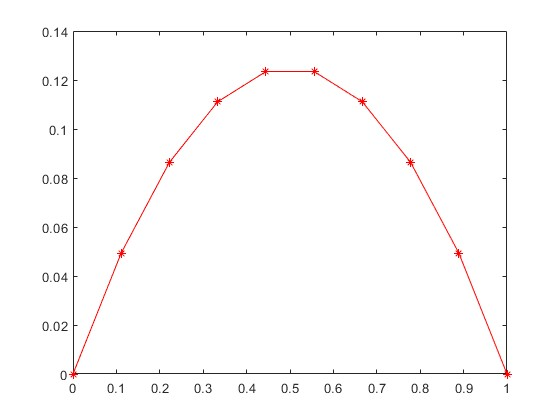
\includegraphics[width=0.9\linewidth]{ones_FEMSol.jpg}
\end{minipage}%
\begin{minipage}{0.5\textwidth}
  \centering
  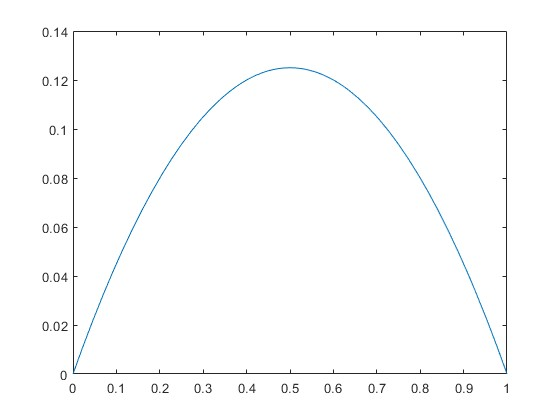
\includegraphics[width=0.9\linewidth]{exact_sol_1.jpg}
\end{minipage}
\caption{Solução aproximada $u_h$ obtida por M.E.F quando $f(x)=1$ e n=10 (gráfico à esquerda) em comparação com a solução exata $u(x)=\frac{1}{2}(1-x)x$ (gráfico à direita).}
\end{figure}

\vspace{5mm}

\tab Como foi referido anteriormente, este código serve de base para o método dos elementos finitos em \textbf{1D}, no sentido em que é possível reproduzir soluções para outros problemas manipulando algumas linhas de código deste \emph{script}. Por exemplo: alterar o número de elementos variando o parâmetro \verb +N+;  definir outra função fonte alterando o conteúdo da linha \verb+f = @(x) ( )+; modificar as condições de fronteira, obtendo outro problema, mas cuja resolução numérica segue os passos da forma fraca do problema de Poisson ou; escolher outro espaço de elementos finitos, ou seja, modificar as funções teste \verb +phi+ e \verb+dphi+. 
Neste sentido, e para efeitos ilustrativos, escolhe-se o espaço de elementos finitos de segundo grau $V_h^2$, que sem considerar condições de fronteira é definido da seguinte forma: $\hat{V}_h^2:=\{u \in C[0,1] \; | \; u|I_i \in P^2(I_i)\;$ para$\; i=1,\cdots,(N-1)\}$. Escolhemos então uma base em $P^2(I_j)$ que é obtida adicionando à base construída anteriormente para o espaço $V_h$ de funções lineares uma função bolha dada por:

\begin{equation*}
     \hat{\varphi}_j(x) = \begin{cases} $$(x-x_j)(x_{j+1}-x)$$, & \mbox{ se } x\mbox{ $\in I_j$} \\ 0, & \mbox{caso contrário}
     \end{cases}
\end{equation*}

\vspace{5mm}

Assim, e usando a quadratura numérica anterior, o \emph{script} passa a ter a seguinte forma:

\vspace{5mm}

\begin{lstlisting}[frame=single]
clear all
clf

% Criacao da particao [0,1]

N = 10;
dim=2*N-1;
p = linspace(0,1,N);

% Nesta expressao podemos fazer a manipulacao de f%
f = @(x) ( sin(x) );

Ahat = sparse(dim,dim);
bhat = zeros(dim,1);

for k=1:(N-1)
    x1 = p(k);
    x2 = p(k+1);
    %function handle porque vamos estar sempre a avaliar
    phi{:,1} = @(x) (x-x2)./(x1-x2);
    phi{:,2} = @(x) (x-x1)./(x2-x1);
    phi{:,3} = @(x) (x-x1).*(x2-x); %funcao bolha%

    dphi{:,1} = @(x)  1/(x1-x2);
    dphi{:,2} = @(x)  1/(x2-x1);
    dphi{:,3} = @(x) -2*x+x2+x1;

    enum = [k k+1 N+k];
    %Regra de quadratura de Gauss
    [X,W]=gaussint(2,p(k),p(k+1),1);

    for i=1:3
        for l=1:2
            bhat(enum(i))=bhat(enum(i))+W(l)*f(X(l))*phi{i}(X(l));
        end
        for j=1:3
            for l=1:2
                Ahat(enum(i),enum(j))= Ahat(enum(i),enum(j))+W(l)*dphi{i}(X(l))*dphi{j}(X(l));
            end
        end
    end
end

idof = setdiff(1:(2*N-1),[1 N]);
A = Ahat(idof,idof);
b = bhat(idof,1);
u(idof) = A\b;


figure(1)
hold on;

% Plot da solucao com bolha
for k=1:N-1
    x1 = p(k);
    x2 = p(k+1);
    phi{:,1} = @(x) (x-x2)./(x1-x2);
    phi{:,2} = @(x) (x-x1)./(x2-x1);
    phi{:,3} = @(x) (x-x1).*(x2-x);
    t = linspace(p(k),p(k+1));
    plot(t,phi{1}(t)*u(k)+phi{2}(t)*u(k+1)+phi{3}(t)*u(k+N));
end
hold off;

figure(2)
hold on;

% Plot da solucao sem bolha
for k=1:N-1
    x1 = p(k);
    x2 = p(k+1);
    phi{:,1} = @(x) (x-x2)./(x1-x2);
    phi{:,2} = @(x) (x-x1)./(x2-x1);
    t = linspace(p(k),p(k+1));
    plot(t,phi{1}(t)*u(k)+phi{2}(t)*u(k+1));
end
ylim([0 0.07]);
hold off;
\end{lstlisting}

\vspace{5mm}

\begin{figure} [H]
\centering
\begin{minipage}{0.5\textwidth}
  \centering
  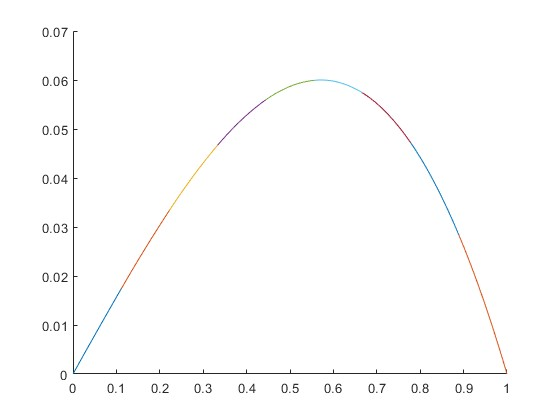
\includegraphics[width=0.9\linewidth]{sin_bolha.jpg}
\end{minipage}%
\begin{minipage}{0.5\textwidth}
  \centering
  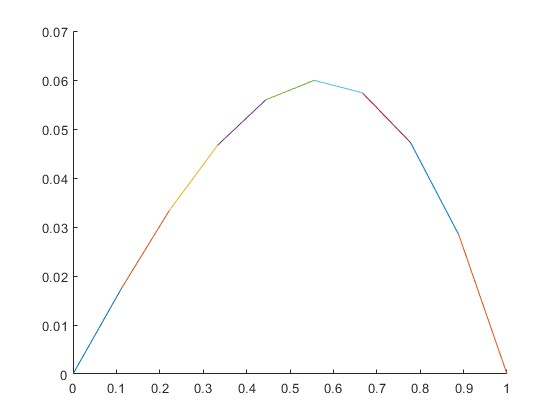
\includegraphics[width=0.9\linewidth]{sin_linear.jpg}
\end{minipage}
\caption{Soluções aproximadas obtidas em $V_h^2$ (gráfico à esquerda) e em $V_h$ (gráfico à direita). As cores representam os diferentes elementos.}
\end{figure}

Como é possível observar, a utilização de elementos quadráticos "suaviza" a curva, o que remete para o facto de a inclusão da função bolha levar a menores erros. Esta questão será aprofundada na secção seguinte.

\vspace{5mm}
\subsection{Análise do erro empírico em 1D}
\tab É agora feita uma análise empírica do erro, isto é, estudamos o erro de solução aproximada comparando-a com a solução explícita conhecida. Definindo uma partição uniforme do intervalo, usa-se o seguinte código \emph{MATLAB} para observar a influência do tamanho do passo $h$ no erro. É de notar que foi criada uma função auxiliar \verb +solver1D+, que corresponde ao código anterior para a assemblagem linear mas adaptado ao formato \verb+function+.

\vspace{5mm}

\begin{lstlisting}[frame=single]
% Codigo adaptado do Professor Antti Hannukainen da Universidade de Aalto [1]

clear all
clf

% Lista das particoes
N_list = [5 10 20 40];

f=@(x)(1+0*x);

t=linspace(0,1,100);

figure(1);
% O comando interpl faz a interpolacao do vetor u da solucao aproximada
for i=1:length(N_list)
    x = linspace(0,1,N_list(i));

    u = solver1D(f,x);

    uh_t=interp1(x,u,t);

    u_t=(1/2)*t.*(1-t);
    
    plot(t,u_t-uh_t);hold on;
end
legend('N=5','N=10','N=20','N=40');
\end{lstlisting}

\vspace{5mm}

Executando este \emph{script} são obtidas as seguintes comparações entre as soluções aproximadas e a solução exata da função constante $f(x)=1$ para um número de elementos progressivamente maior:


\begin{figure}[H]
\centering
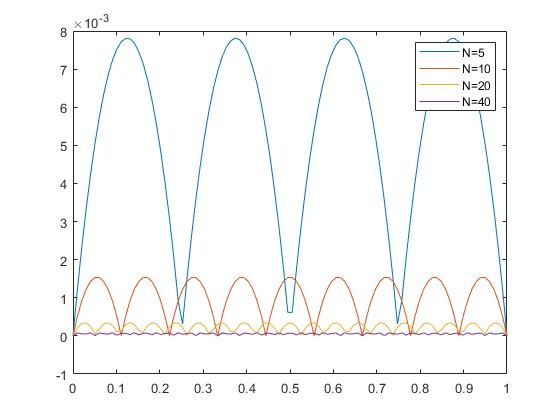
\includegraphics[scale=0.5]{erro_h.jpg}
\caption{Função erro $e$ versus o número de partições $N$.}
\end{figure}

Observando a Figura 3 conclui-se que o aumento do número de elementos leva a uma diminuição substancial do erro.

\vspace{5mm}

\tab É possível também quantificar os erros pela sua norma associada. Para tal, é necessário reparar que para a restrição $e|I_j = u|I_j - u_h|I_j$ se tem $u_h|I_j = \hat{\beta}_j\hat{\varphi}_j|I_j + \hat{\beta}_{j+1}\hat{\varphi}_{j+1}|I_j$ em que $\hat{\beta}_j$ e $\hat{\beta}_{j+1}$ são, respetivamente, a $j$-ésima e $\{j+1\}$-ésima coordenadas do vetor:
\begin{equation*}
    \hat{\beta}=\begin{bmatrix} 0 \\ \beta \\ 0\end{bmatrix}
\end{equation*}
 Considerando  as normas $L^2(0,1)$, $H^1(0,1)$ e a norma de energia $E(0,1)$, então, usando, novamente, a regra de quadratura de Gauss de dois pontos tal que $\norm{e}\approx \sum^2_{k=1} e(t_k)\cdot w_k$, em que $t$ é o vetor de pontos de integração e $w$ o vetor de pesos, temos o seguinte código \emph{MATLAB}:

\vspace{5mm}

\begin{lstlisting}[frame=single]
function [L2error,Eerror,Herror] = erro_fem1D_linear(x,u,ufun,dufun)
% Devolve as respetivas normas
    % Valores para as normas
    val_L2=0;
    val_E=0;
    val_H=0;
    for i=1:(length(x)-1)
        % Regra de Quadratura de Gauss
        [t,w] = gaussint(2,x(i),x(i+1));
        % Pontos avaliados
        uh_tk = zeros(1,length(t));
        duh_tk = zeros(1,length(t));
        u_tk = zeros(1,length(t));
        du_tk = zeros(1,length(t));
            for k=1:length(t)
                uh_tk(k) = u(i)*( x(i+1)-t(k))/(x(i+1)-x(i));
                uh_tk(k) = uh_tk(k) + u(i+1)*( x(i)-t(k))/(x(i)-x(i+1));
                duh_tk(k) = -u(i)/(x(i+1)-x(i));
                duh_tk(k) = duh_tk(k) - u(i+1)/(x(i)-x(i+1));
                u_tk(k) = ufun(t(k));
                du_tk(k) = dufun(t(k));
            end
        val_L2 = val_L2 + (u_tk - uh_tk).^2*w(:);
        val_E = val_E + (du_tk - duh_tk).^2*w(:);
        val_H = val_H + (u_tk - uh_tk).^2*w(:) + (du_tk - duh_tk).^2*w(:) ;
    end
    L2error = sqrt(val_L2);
    Eerror = sqrt(val_E);
    Herror = sqrt(val_H);
end
\end{lstlisting}
\vspace{5mm}

Escolhendo agora uma função definida por ramos $f$ tal que:

\begin{equation*}
     f(x) = \begin{cases} \;-1, & \mbox{ se } x\mbox{ $\in [0,\frac{1}{2}]$} \\ \; 1, & \mbox{ se }  x\mbox{ $\in (\frac{1}{2},1] $}
     \end{cases}
\end{equation*}

Neste caso a solução explícita é dada por:

\begin{equation*}
     u(x) = \begin{cases} \; \frac{1}{2}x^2 - \frac{1}{4}x, & \mbox{ se } x\mbox{ $\in [0,\frac{1}{2}]$} \\ \; -\frac{1}{2}(x-1)^2 - \frac{1}{4}(x-1), & \mbox{ se }  x\mbox{ $\in (\frac{1}{2},1] $}
     \end{cases}
\end{equation*}

e a sua primeira derivada é:

\begin{equation*}
     u'(x) = \begin{cases} \; x - \frac{1}{4}, & \mbox{ se } x\mbox{ $\in [0,\frac{1}{2}]$} \\ \;  -x  + \frac{3}{4}, & \mbox{ se }  x\mbox{ $\in (\frac{1}{2},1] $}
     \end{cases}
\end{equation*}
\vspace{1mm}

\tab É importante realçar que a primeira derivada de $u$ é contínua mas a segunda não é, pelo que $u$ não satisfaz a formulação forte do problema de Poisson mas satisfaz a formulação variacional (fraca), isto é, $u \in H_0^1(0,1)$.

Calcula-se, então, o erro da solução aproximada por elementos finitos em função do tamanho de $h$ através do seguinte \emph{script}:

\vspace{1mm}

\begin{lstlisting}[frame=single]
clear all;
N_list = [10 20 40 80 160 320];
f=@(x) (-1).*(x<=1/2)+(1).*(x>1/2);
e=@(x) ((1/2)*x^2-(1/4)*x).*(x<=1/2)+(-(1/2)*(x-1)^2-(1/4)*(x-1)).*(x>1/2);
de=@(x) (x-(1/4)).*(x<=1/2)+(-(x)+1-(1/4)).*(x>1/2);
for i = 1:length(N_list)
    x = linspace(0,1, N_list(i) );
    u = solver1D(f,x);
    [L2error(i),Eerror(i),Herror(i)] = erro_fem1D_linear(x,u,e,de);
end

figure(1)
loglog(1./(N_list-1),L2error,'k:o');
hold on;
loglog(1./(N_list-1),1./(N_list-1).^2,'--or');
legend({'Erro na norma L2','Taxa de h^2'},'Location','northwest')
xlabel('Tamanho da Particao')
hold off;

figure(2)
loglog(1./(N_list-1),Eerror,'k:o');
hold on;
loglog(1./(N_list-1),1./(N_list-1),'--or');
legend({'Erro na norma E','Taxa de h'},'Location','northwest')
xlabel('Tamanho da Particao')
hold off;

figure(3)
loglog(1./(N_list-1),Herror,'k:o');
hold on;
loglog(1./(N_list-1),1./(N_list-1),'--or');
legend({'Erro na norma H^1','Taxa de h'},'Location','northwest')
xlabel('Tamanho da Particao')
hold off;

\end{lstlisting}
\vspace{5mm}

Os resultados em diferentes normas são apresentados nas Figuras 4, 5 e 6.

\begin{figure}[H]
\centering
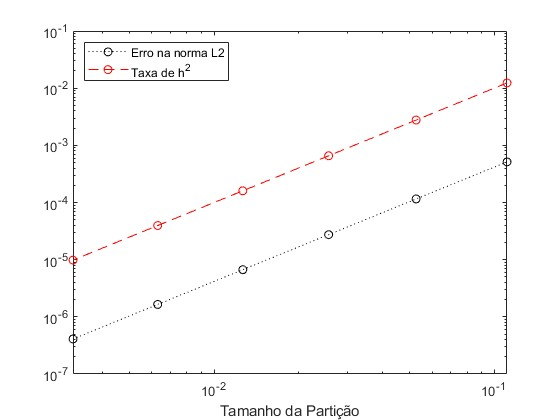
\includegraphics[scale=0.4]{linear_normL.jpg}
\caption{Gráfico \textbf{loglog} da norma $L^2(0,1)$ versus $h$. }
\end{figure}

\begin{figure}[H]
\centering
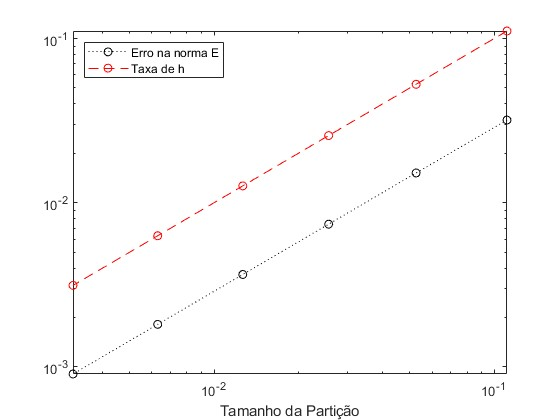
\includegraphics[scale=0.4]{linear_normE.jpg}
\caption{Gráfico \textbf{loglog} da norma de energia $E(0,1)$ versus $h$. }
\end{figure}

\begin{figure}[H]
\centering
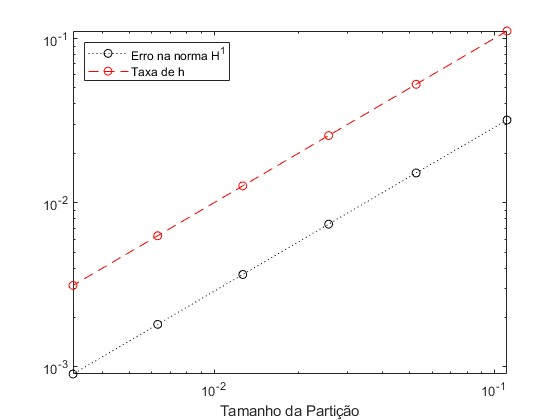
\includegraphics[scale=0.4]{linear_normH.jpg}
\caption{Gráfico \textbf{loglog} da norma $H^1(0,1)$ versus $h$.}
\end{figure}

\vspace{1mm}

\tab Desta forma, confirmam-se os resultados teóricos da secção 2.3. Efetivamente, relembrando que a transformação \textbf{loglog} satisfaz $log(y)=klog(x)+b$ tal que $y=10^{klog(x)+b}=Cx^k$, é possível estabelecer uma relação direta entre o declive da reta no gráfico \textbf{loglog} e a convergência $O(h^k)$ das normas. Assim sendo, olhando para a Figura 4, conclui-se que a norma $L^2(0,1)$ se comporta como $Ch^2$ para uma dada constante $C$. Observando a Figura 5 e a Figura 6, é possível deduzir que as normas $E(0,1)$ e $H^1(0,1)$ se comportam como $Ch$.

\tab No caso dos elementos finitos da segunda ordem, modificando tanto o \emph{script} anterior como a função \emph{solver1D} para acomodar a inclusão da função bolha, escolhendo a função $f(x)=sin(\pi x)$ com solução exata $u(x)=\frac{sin(\pi x)}{(\pi^2)}$ e derivada $u'(x)=\frac{cos(\pi x)}{\pi}$ obtêm-se as imagens subsequentes:

\begin{figure}[H]
\centering
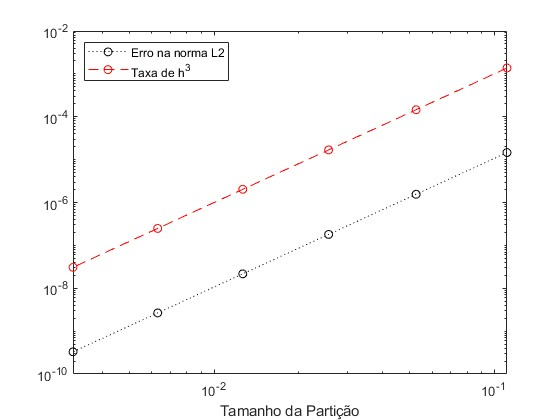
\includegraphics[scale=0.4]{bubble_normL.jpg}
\caption{Gráfico \textbf{loglog} da norma $L^2(0,1)$ em $V_h^2$ versus $h$. }
\end{figure}

\begin{figure}[H]
\centering
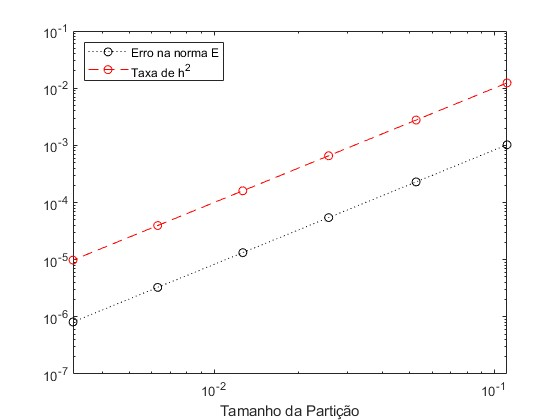
\includegraphics[scale=0.4]{bubble_normE.jpg}
\caption{Gráfico \textbf{loglog} da norma de energia $E(0,1)$ em $V_h^2$ versus $h$. }
\end{figure}

\begin{figure}[H]
\centering
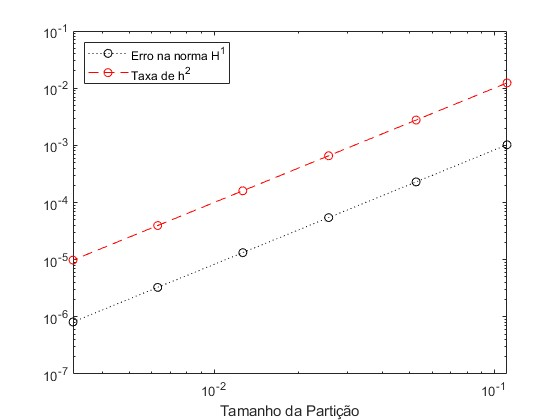
\includegraphics[scale=0.4]{bubble_normH.jpg}
\caption{Gráfico \textbf{loglog} da norma $H^1(0,1)$ em $V_h^2$ versus $h$.}
\end{figure}

\vspace{5mm}

\tab Usando o raciocínio do parágrafo anterior, conclui-se que para este escolha de espaço de funções base a norma $L^2(0,1)$ se comporta como $Ch^3$ e as normas $E-norm$ e $H^1(0,1)$ se comportam como $Ch^2$, aumentando, portanto, um grau na ordem de convergência. Assim sendo, a estipulação prévia de que o uso de um espaço de segundo grau leva a menores erros é confirmada.

\section{Implementação do M.E.F em 2D}
\subsection{Assemblagem do sistema linear em 2D}
\tab O primeiro passo para obter a solução aproximada, com condição de Dirichlet nula, num domínio $\Omega \subset \mathbb{R}^2$ é criar uma malha triangular (ou quadrilateral) definida pela matriz $p \in \R^{2 \times \N_p}$, que contém os $p$ nós (ou nodos) da triangulação, e pela matriz $t \in \N^{3 \times N_t}$, que contém os indíces dos vértices dos $N_t$ triângulos. Estas matrizes podem ser introduzidas de forma manual ou, a fim de obter triangulações mais complexas, usando funções auxiliares disponibilizadas pela biblioteca \verb +pde toolbox+. Por curiosidade foram escolhidas três malhas: uma quadrada; outra rectangular; e uma em forma L. Seguidamente foi aplicada a função \verb +solver2D+ que calcula a solução aproximada para uma dada função fonte $f$, neste exemplo $f(x,y)=sin(\pi x)sin(\pi y)$, que também recebe como argumentos a malha e o parâmetro de refinamento $N$. As funções responsáveis pela geração da malha, \verb +inittri(p,t)+, pelo refinamento, \verb +refine_tri(mesh)+, e pela regra de quadratura triangular, \verb +inttri(p)+, foram obtidas das notas do Professor Antti Hannukainen da Universidade de Aalto \textbf{[1]}.

\vspace{5mm}
\begin{lstlisting}[frame=single]
clear all
% funcao source
% Os valores de N indicam o numero de vezes a refinar a malha
f = @(x,y)(sin(pi.*x).*sin(pi.*y));

% Criar triangulacao em mesh retangular
N=6;
p = [ 0 10 10 0 ; 0 0 10 10];
t = [ 1 2 3; 1 4 3]';
mesh1=make_mesh(N,p,t);

solver2D(f,N,mesh1);

% Criar triangulacao em mesh exemplo
N=5;
p =[ 0 1 2 0 1 2 ; 0 0 0 1 1 1];
t = [ 1 2 2 3 ; 2 4 3 5 ; 4 5 5 6 ];
mesh2=make_mesh(N,p,t);

solver2D(f,N,mesh2);

% Criar triangulacao em mesh L
N=1;
model = createpde(1);
geometryFromEdges(model,@lshapeg);
lshape=generateMesh(model);
mesh3=make_mesh(N,lshape.Nodes,lshape.Elements);

solver2D(f,N,mesh3);

% Criar triangulacao em mesh Test
N=1;
model = createpde(1);
g = geometryFromEdges(model,@cardg);
testshape=generateMesh(model);
mesh4=make_mesh(N,testshape.Nodes,testshape.Elements);

solver2D(f,N,mesh4);
\end{lstlisting}
\vspace{10mm}

\tab Cada uma das seguintes Figuras (10-13) contém: uma imagem da solução aproximada na própria triangulação, em que o gradiente de cores ilustra o afastamento do plano $z=0$ , e; uma visualização da solução em três dimensões.

\vspace{10mm}

\begin{figure} [H]
\centering
\begin{minipage}{0.5\textwidth}
  \centering
  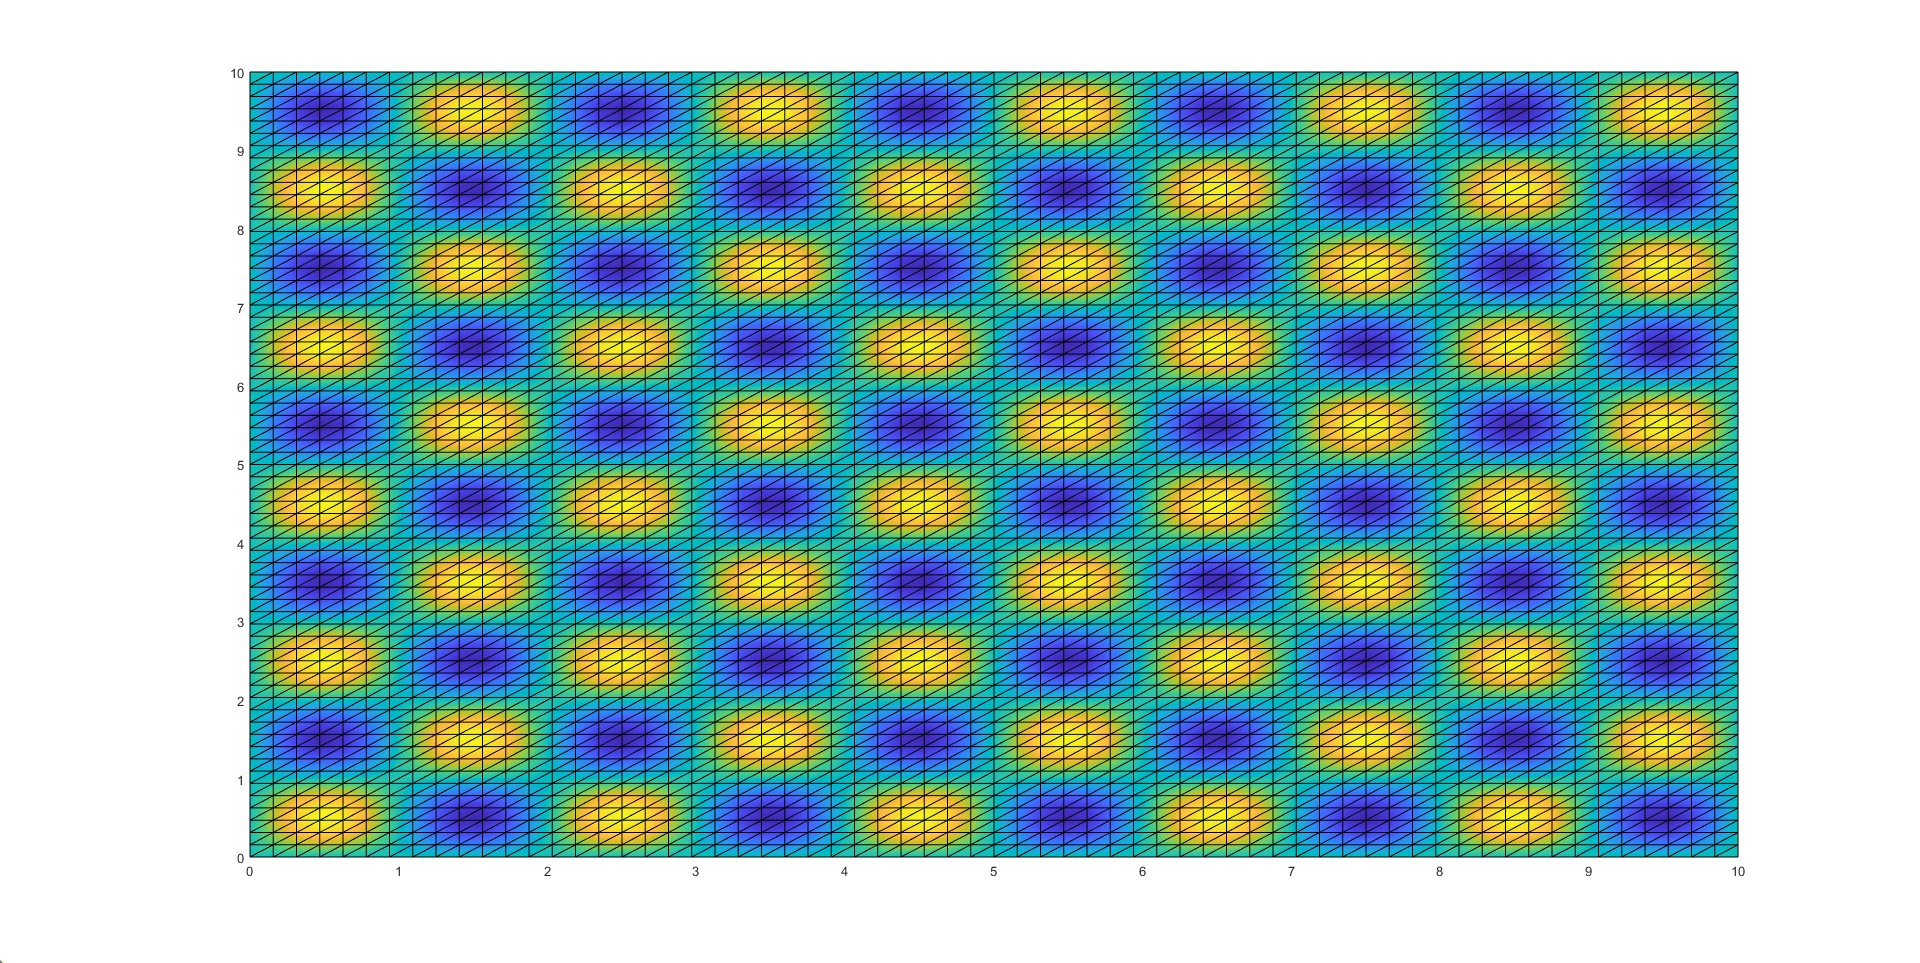
\includegraphics[width=5cm,height=5cm]{sol_grad_rect.jpg}
\end{minipage}%
\begin{minipage}{0.5\textwidth}
  \centering
  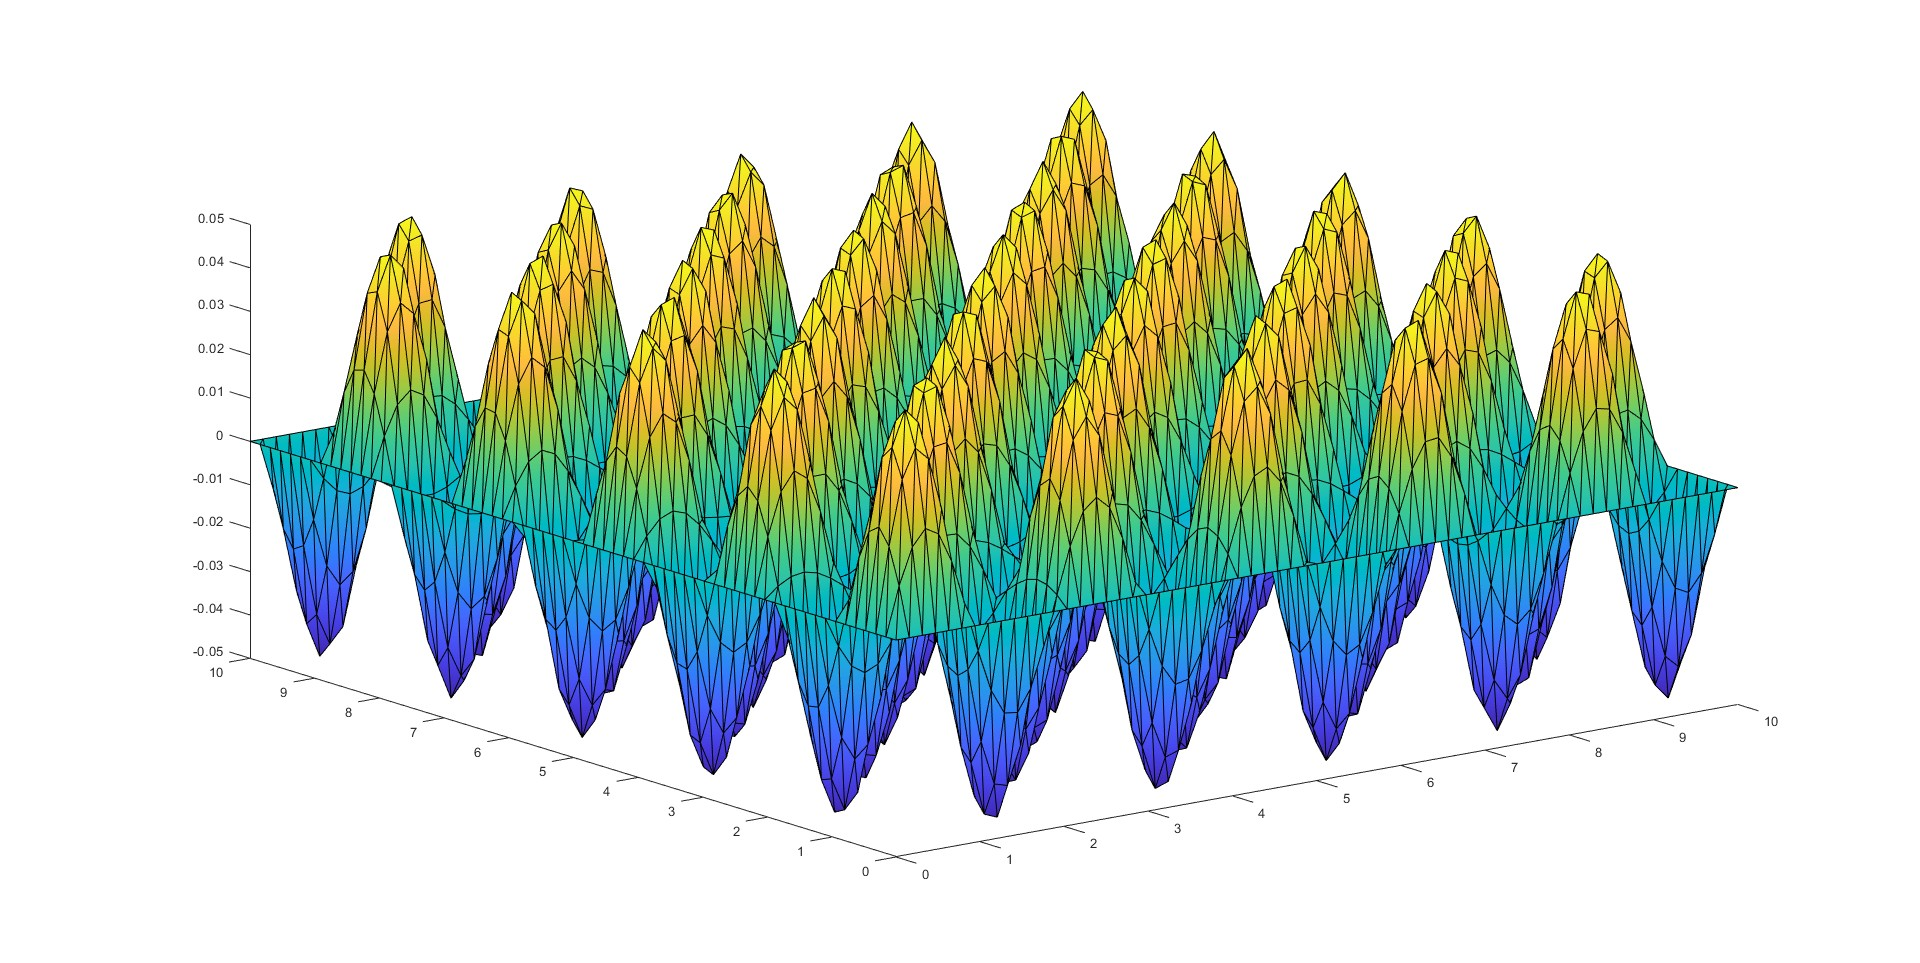
\includegraphics[width=5cm,height=5cm]{sol_rect.jpg}
\end{minipage}
\caption{ Malha quadrada $ [0, 10] × [0, 10] $ com seis refinamentos e solução aproximada.}
\end{figure}


\vspace{15mm}

\begin{figure} [H]
\centering
\begin{minipage}{0.5\textwidth}
  \centering
  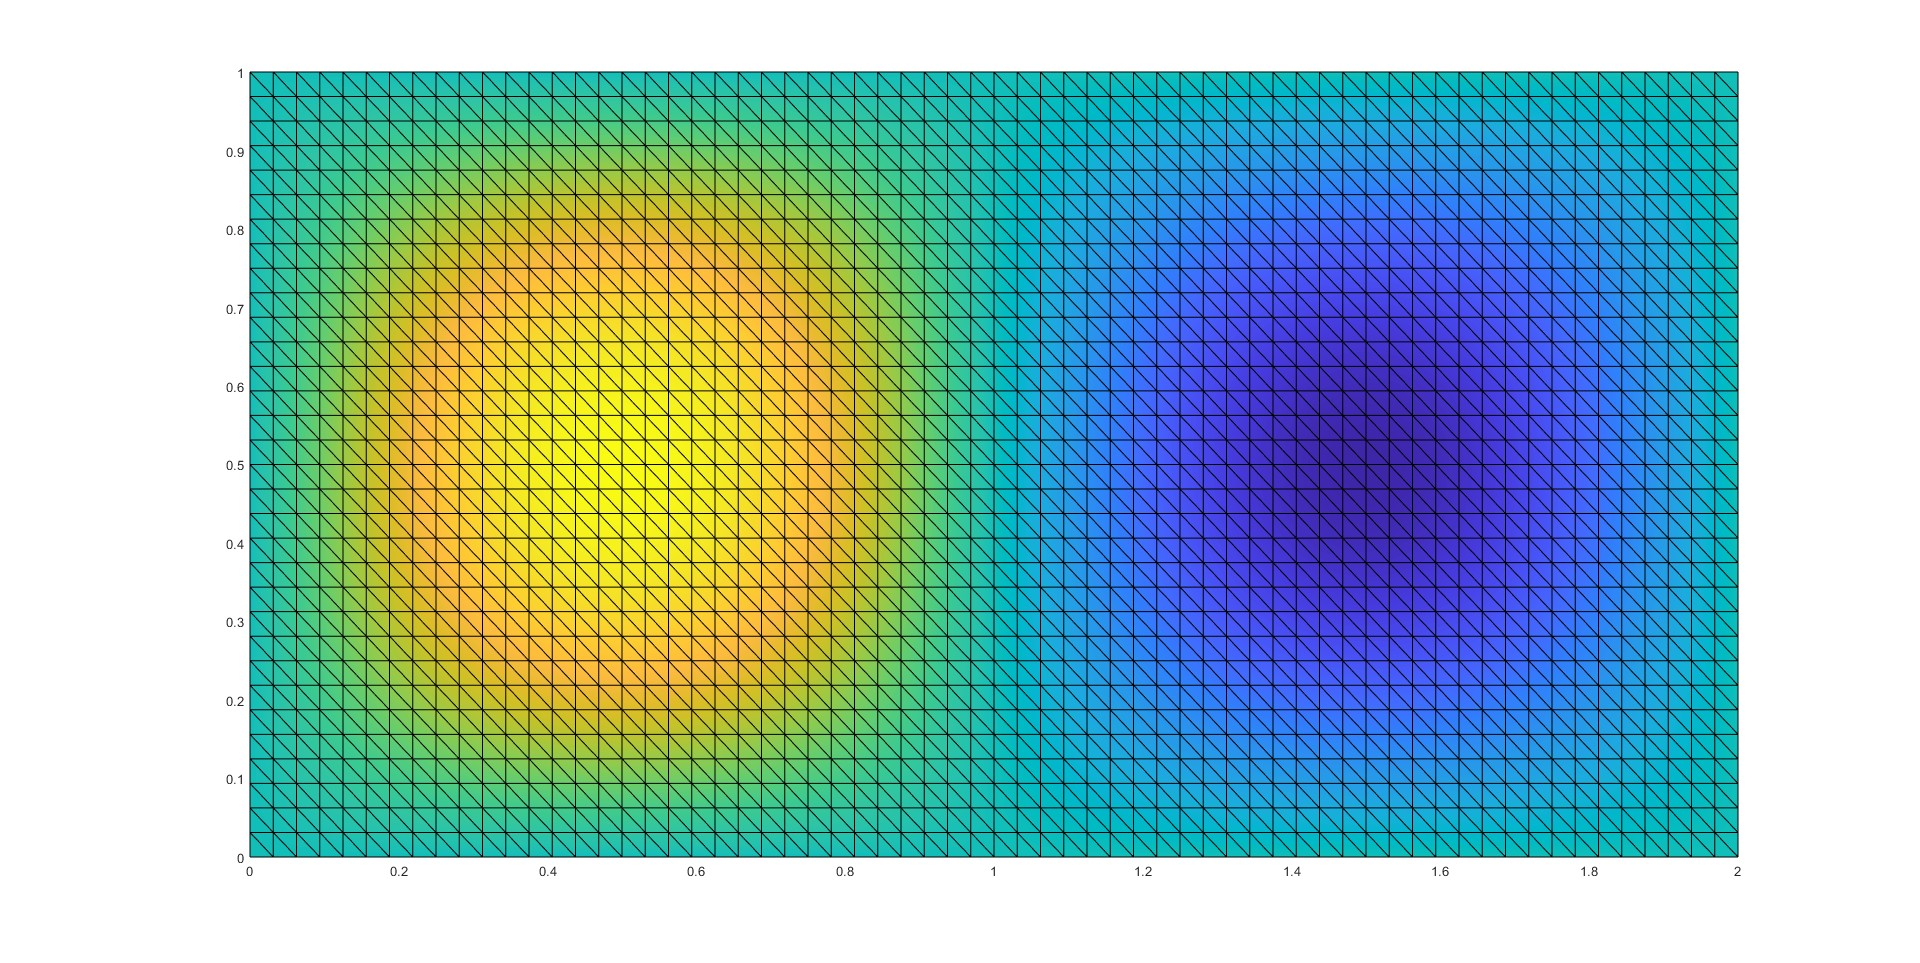
\includegraphics[width=5cm,height=2.5cm]{sol_grad_exemplo.jpg}
\end{minipage}%
\begin{minipage}{0.5\textwidth}
  \centering
  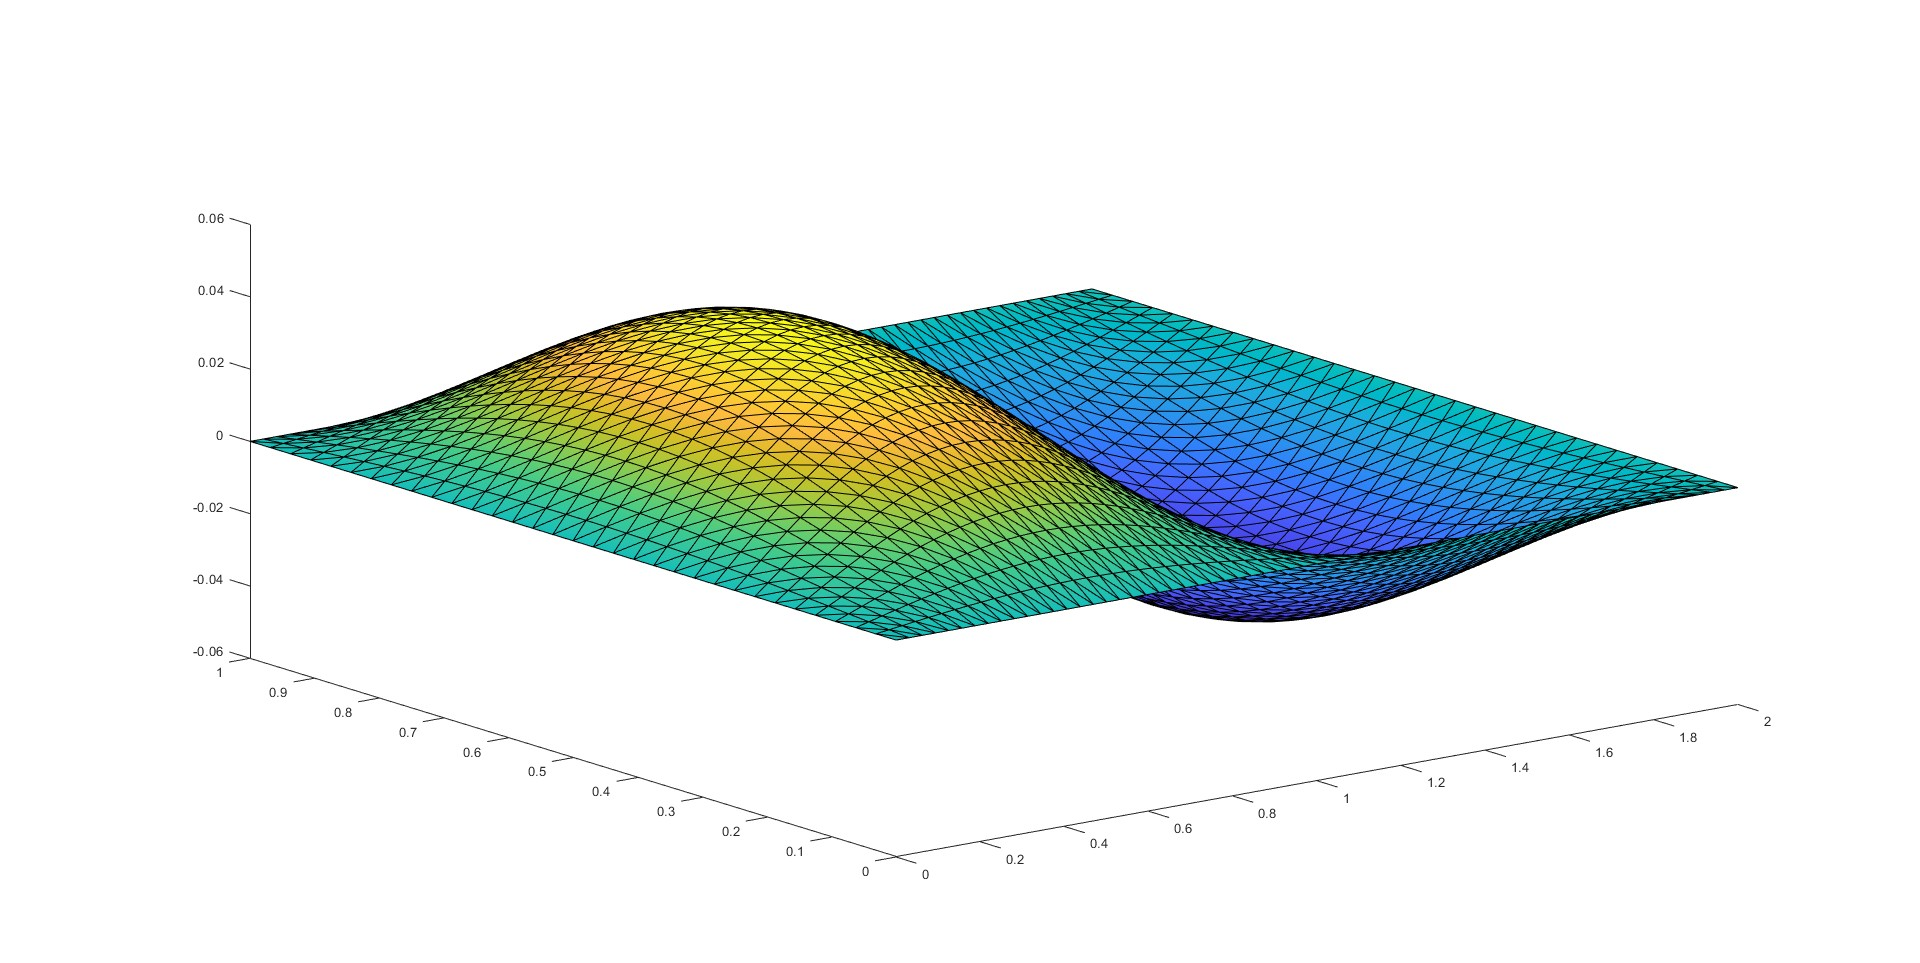
\includegraphics[width=5cm,height=2.5cm]{sol_exemplo.jpg}
\end{minipage}
\caption{ Malha quadrada rectangular $ [0, 2] × [0, 1] $ com cinco refinamentos e solução aproximada.}
\end{figure}

\vspace{15mm}

\begin{figure} [H]
\centering
\begin{minipage}{0.5\textwidth}
  \centering
  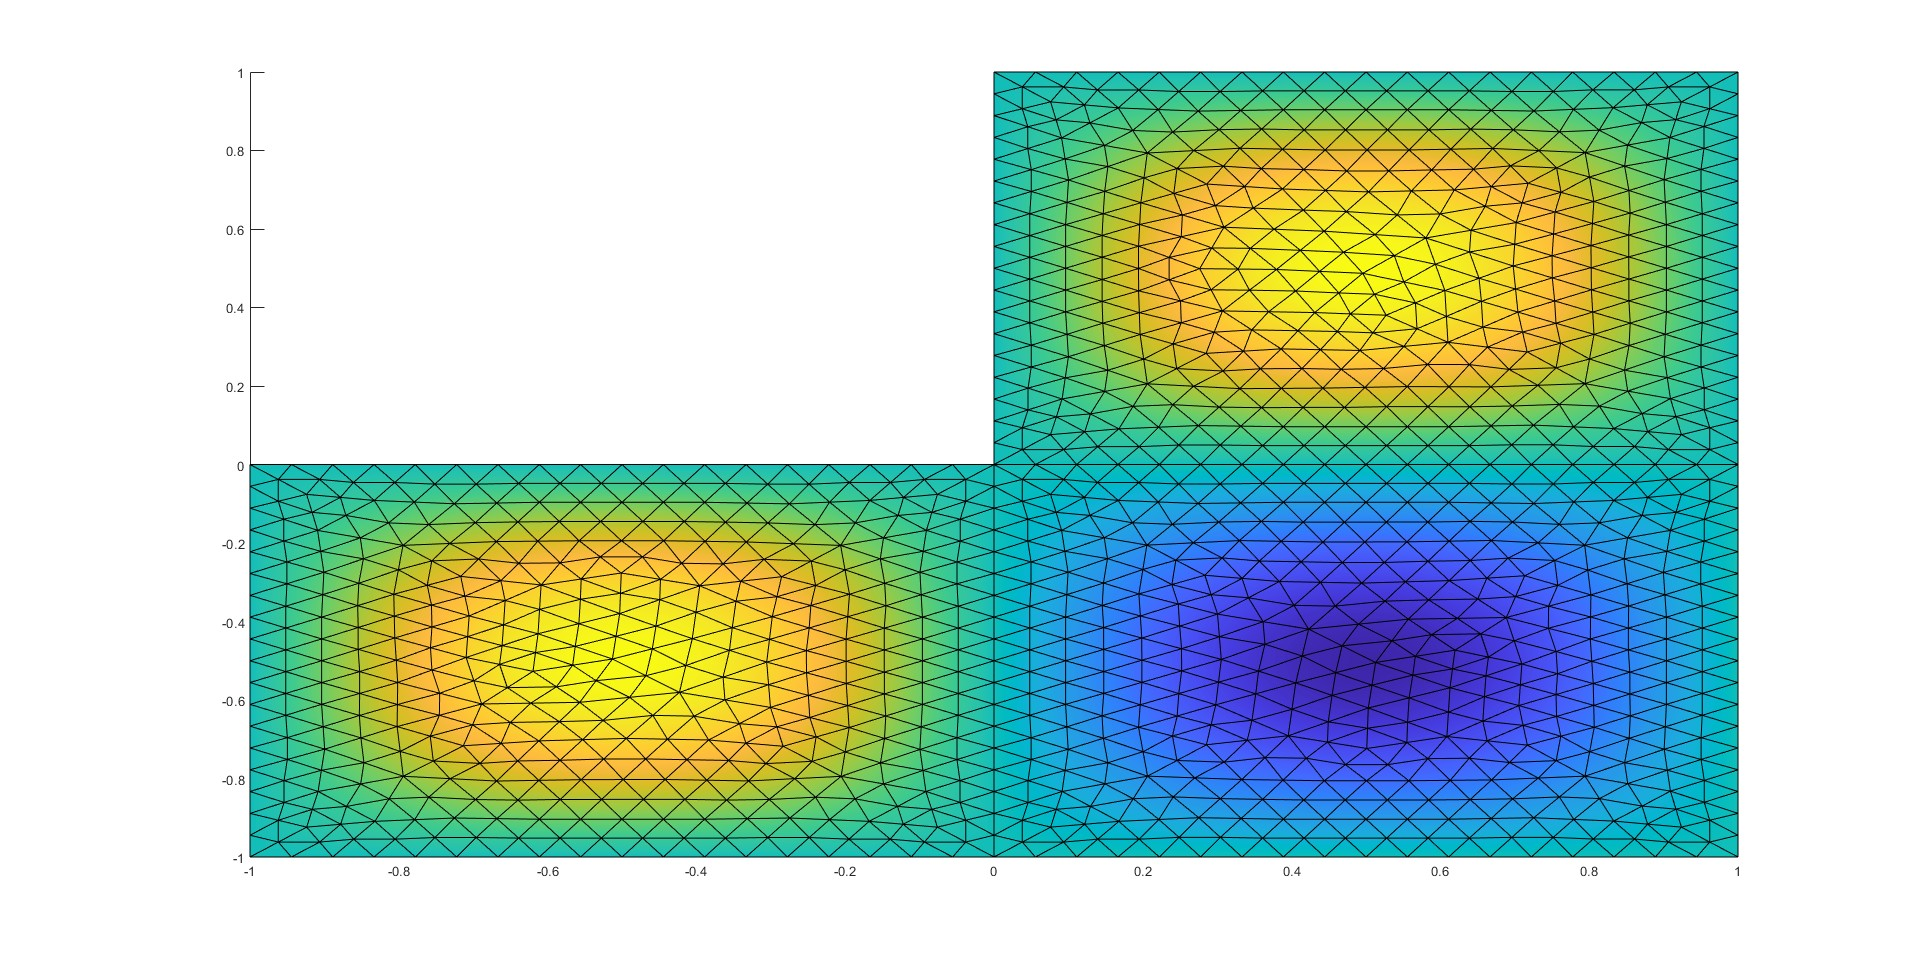
\includegraphics[width=5cm,height=5cm]{sol_grad_L.jpg}
\end{minipage}%
\begin{minipage}{0.5\textwidth}
  \centering
  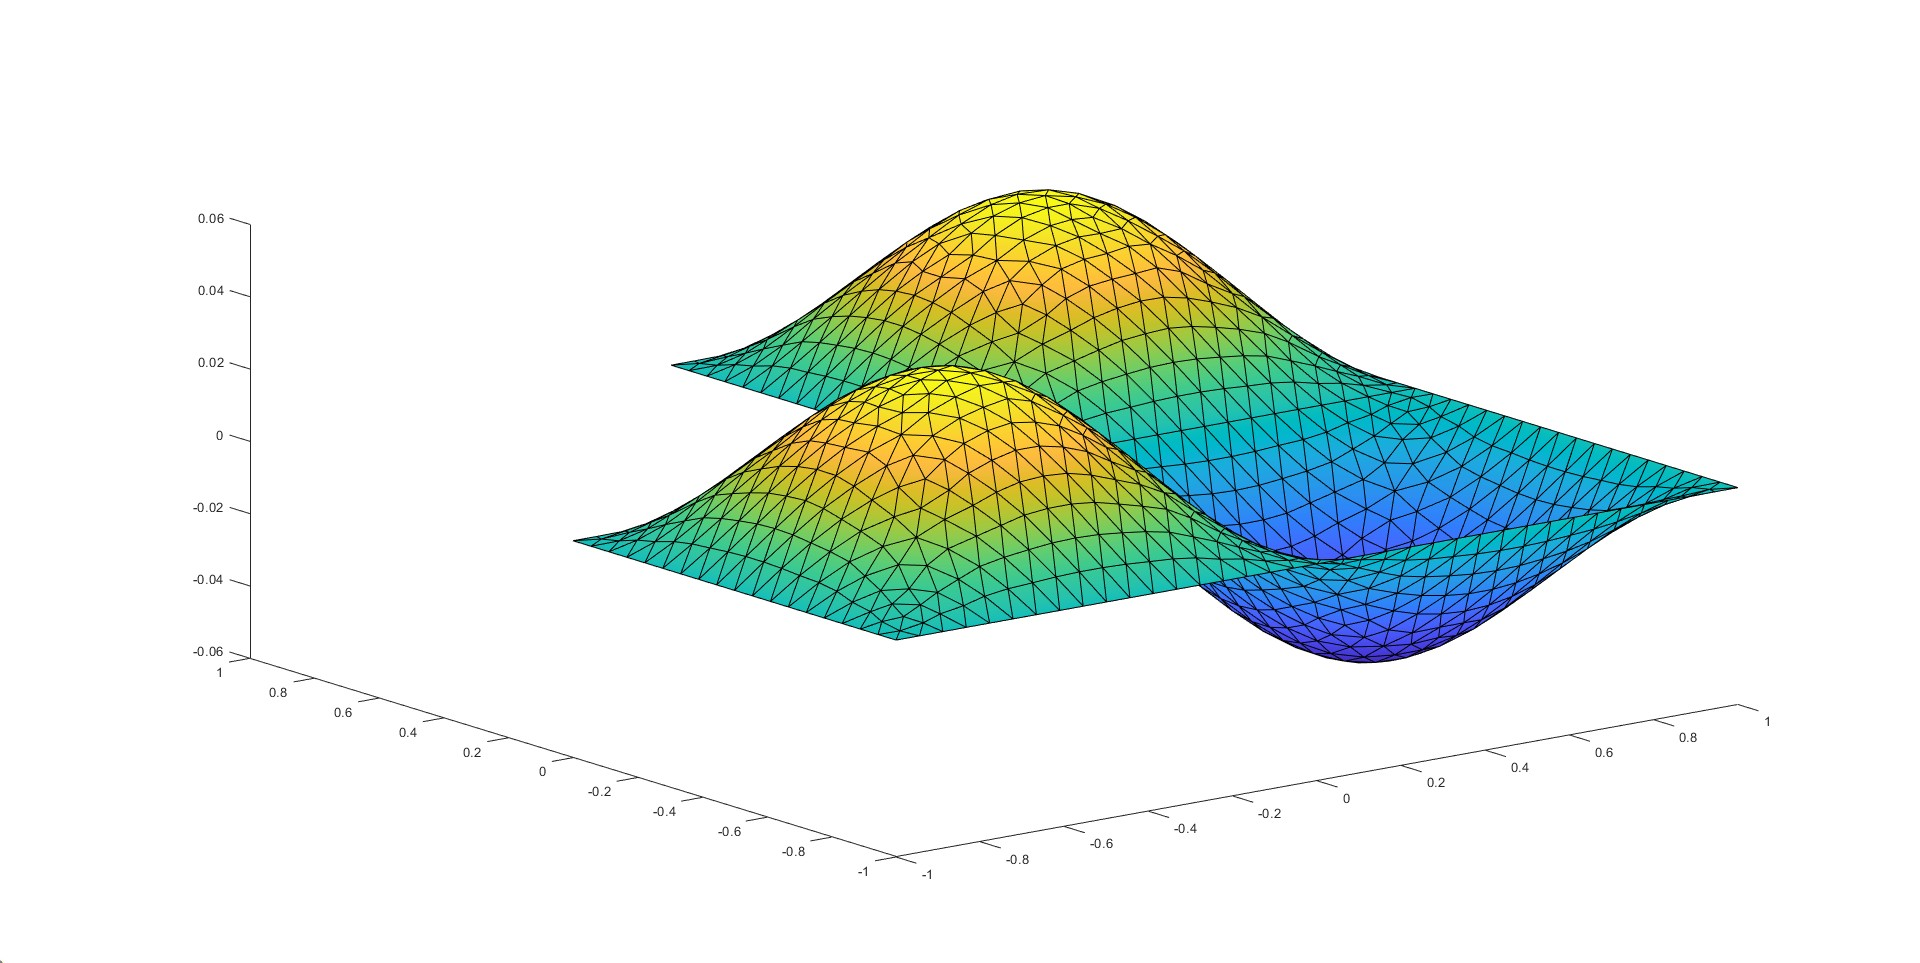
\includegraphics[width=5cm,height=5cm]{sol_L.jpg}
\end{minipage}
\caption{ Malha em forma L no quadrado $[0, 1] \times [0, 1]$ e solução aproximada.}
\end{figure}


\vspace{10mm}

\tab O código da função \emph{solver2D} segue os passos indicados na secção 2.5 para assemblagem da solução aproximada em \textbf{2D}.

\vspace{5mm}
\begin{lstlisting}[frame=single]
function [u] = solver2D(f,N,mesh)
    T=mesh.t;
    P=mesh.p;
    Nt=size(T,2);
    
    bhat=sparse(size(P,2),1);
    Ahat=sparse(size(P,2),size(P,2));
    
    
    for i=1:Nt
        
        % X - Pontos a serem avaliados
        % W - Pesos
        [X,W] = inttri(N);
    
        % Matriz At, vetor bt
    
        At(1,1)=(P(1,T(2,i))-P(1,T(1,i)));
        At(1,2)=(P(1,T(3,i))-P(1,T(1,i)));
        At(2,1)=(P(2,T(2,i))-P(2,T(1,i)));
        At(2,2)=(P(2,T(3,i))-P(2,T(1,i)));
    
        bt(1,1)=P(1,T(1,i));
        bt(2,1)=P(2,T(1,i));
    
        % Calculo det
        detAt=det(At);
    
        % Derivadas
        Nip=size(X,2);
        dL{1} = [ -ones(1,1); -ones(1,1) ];
        dL{2} = [  ones(1,1); zeros(1,1) ];
        dL{3} = [ zeros(1,1);  ones(1,1) ];
    
        for l=1:3
            for j=1:Nip
                % Avaliacao das bases
                phi(:,1) = 1-X(1,j)-X(2,j);
                phi(:,2) = X(1,j);
                phi(:,3) = X(2,j);
                
                % Avaliacao de Ft 
                Xhat(1,1)=X(1,j);
                Xhat(2,1)=X(2,j);
        
                Ft=(At*Xhat)+bt;
    
                bhat(T(l,i))=bhat(T(l,i))+f(Ft(1),Ft(2))*phi(l)*abs(detAt)*W(j);
            end
            for k=1:3
                Ahat(T(l,i),T(k,i))=Ahat(T(l,i),T(k,i))+0.5*transpose(dL{l})*inv(At)*transpose(inv(At))*dL{k}*abs(detAt);
            end
       end
    end

    
    % Pontos de interior e fronteira
    be = find( mesh.e2t(2,:) == 0);
    bind = mesh.edges(:,be);
    bind = unique(bind(:));
    iind = setdiff(1:size(mesh.p,2),bind);

    u =zeros( size(mesh.p,2),1);
    u(iind) = Ahat(iind,iind)\bhat(iind);
    X = mesh.p(1,:);
    Y = mesh.p(2,:);
    t = mesh.t;
    
    figure
    plot_2Dtri_mesh(mesh)
    
    figure
    patch(X(t),Y(t),u(t),u(t));
    view(3);
end
\end{lstlisting}
\vspace{5mm}

\tab Para efeitos de visualização da Figura 14 mostra-se a diferença entre a solução obtida por M.E.F e a solução exata em $\Omega=(0,1)^2$ da função $f(x,y)=2y(1-y)+2x(1-x)$.

\begin{figure} [H]
\centering
\begin{minipage}{0.5\textwidth}
  \centering
  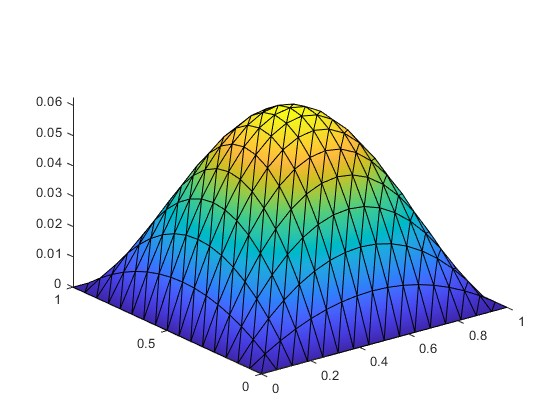
\includegraphics[width=0.9\linewidth]{approx_sol_2.jpg}
\end{minipage}%
\begin{minipage}{0.5\textwidth}
  \centering
  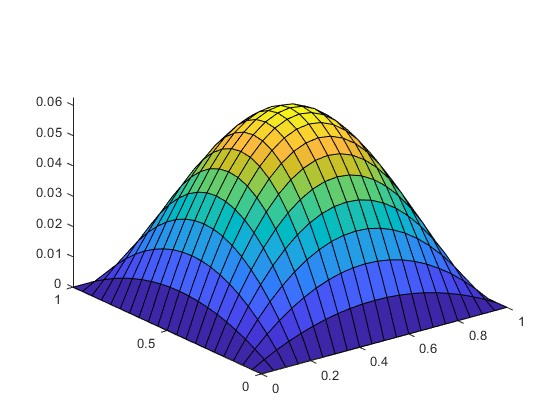
\includegraphics[width=0.9\linewidth]{exact_sol_2.jpg}
\end{minipage}
\caption{Soluções obtida por M.E.F e representação da solução exata $u=x(1-x)y(1-y)   $.}
\end{figure}

\subsection{Análise do erro empírico em 2D}

\tab O estudo dos erros empíricos em \textbf{2D} segue as mesmas ideias introduzidas na secção irmã 3.2. Contudo, dada à dificuldade de arranjar soluções exatas para estas equações, é necessário arranjar outra estratégia: em vez de se considerar a solução exata considera-se uma solução aproximada já com um valor de $h$ muito reduzido. Desta forma, considera-se a seguinte função \verb +erro_FEM2D+ :

\vspace{5mm}

\begin{lstlisting}[frame=single]
 function [L2error, Eerror] = erro_fem2D(mesh,f,uf,u)
% Devolve as respetivas normas
    % Valores para as normas
    val_L2=0;
    val_E=0;
    % Inicializacao das matrizes 
    P=mesh.p;
    T=mesh.t;
    Nt=size(T,2);

    % Bases referencia 
    phi{:,1} = @(x,y) 1-x-y;
    phi{:,2} = @(x,y) x;
    phi{:,3} = @(x,y) y;
    
    

    for i=1:Nt
        % Funcao erro e derivada do erro
        err = @(x,y) (uf(T(1,i))*phi{1}(x,y)+uf(T(2,i))*phi{2}(x,y)+uf(T(3,i))*phi{3}(x,y))-(u(T(1,i))*phi{1}(x,y)+u(T(2,i))*phi{2}(x,y)+u(T(3,i))*phi{3}(x,y));
        derr = @(x,y) f(x,y)*((uf(T(1,i))*phi{1}(x,y)+uf(T(2,i))*phi{2}(x,y)+uf(T(3,i))*phi{3}(x,y))-(u(T(1,i))*phi{1}(x,y)+u(T(2,i))*phi{2}(x,y)+u(T(3,i))*phi{3}(x,y)));
        % Pesos e pontos
        [t,w] = inttri(20);

        % Matriz At, vetor bt e det 
        At(1,1)=(P(1,T(2,i))-P(1,T(1,i)));
        At(1,2)=(P(1,T(3,i))-P(1,T(1,i)));
        At(2,1)=(P(2,T(2,i))-P(2,T(1,i)));
        At(2,2)=(P(2,T(3,i))-P(2,T(1,i)));
    
        bt(1,1)=P(1,T(1,i));
        bt(2,1)=P(2,T(1,i));

        detAt=det(At);
        
        % Loop de regra de quadratura
        for j=1:length(t)
            Xhat(1,1)=t(1,j);
            Xhat(2,1)=t(2,j);
            Ft=(At*Xhat)+bt;
            val_L2=val_L2+(err(Ft(1),Ft(2)))^2*abs(detAt)*w(j);
            val_E=val_E+(abs(derr(Ft(1),Ft(2))))*abs(detAt)*w(j);
        end
    end
    % Avaliacao das normas
    L2error = sqrt(val_L2);
    Eerror = sqrt(val_E);
end

\end{lstlisting}

\vspace{1mm}

Esclarece-se ainda que para a análise do erro na norma de energia se utilizou a igualdade:
\begin{equation*}
    \int_\Omega \abs{\nabla u - \nabla u_h}^2 = \int_\Omega f(u-2u_h) + \int_\Omega fu_h
\end{equation*}

\tab Considerando-se, novamente, a função $f(x,y)=sin(\pi x)sin(\pi y)$ é possível calcular o erro para diferentes valores de $h_T$ através do seguinte script:

\vspace{5mm}

\begin{lstlisting}[frame=single]
clear all;
% Script que produz a norma associada ao erro para varias normas e particoes
N_list = [ 3 4 5 6 7];
f = @(x,y)(sin(pi*x)*sin(pi*y));

p = [ 0 1 1 0 ; 0 0 1 1];
t = [ 1 2 3; 1 4 3]';

% Criacao da malha proxima da solucao
meshy=make_mesh(8,p,t);
uf=solver2D(f,7,meshy);

% Loop de comparacao
for i = 1:length(N_list)
    mesh=make_mesh(N_list(i),p,t);
    h(i)=give_h(mesh);
    u=solver2D(f,N_list(i),mesh);
    [L2error(i),Eerror(i)] = erro_fem2D(mesh,f,uf,u);
end

figure(1)
loglog(h,L2error,'k:o');
hold on;
loglog(h,h.^2,'--or');
legend({'Erro na norma L2','Taxa de h^2'},'Location','northwest')
xlabel('Tamanho de h')
hold off;

figure(2)
loglog(h,Eerror,'k:o');
hold on;
loglog(h,h,'--or');
legend({'Erro na norma E','Taxa de h'},'Location','northwest')
xlabel('Tamanho de h')
hold off;

\end{lstlisting}

\vspace{5mm}

\begin{figure}[H]
\centering
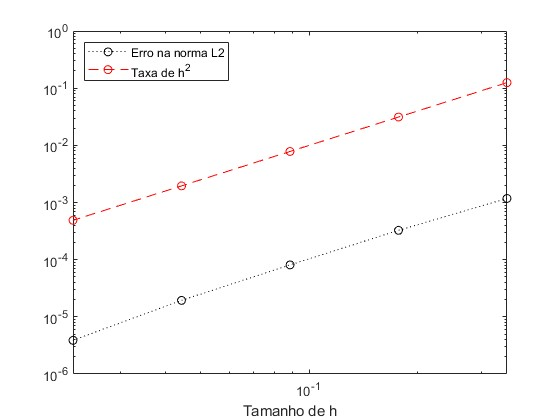
\includegraphics[scale=0.4]{2D_normL.jpg}
\caption{Gráfico \textbf{loglog} da norma $L^2$ na triangulação versus o tamanho de h. }
\end{figure}

\begin{figure}[H]
\centering
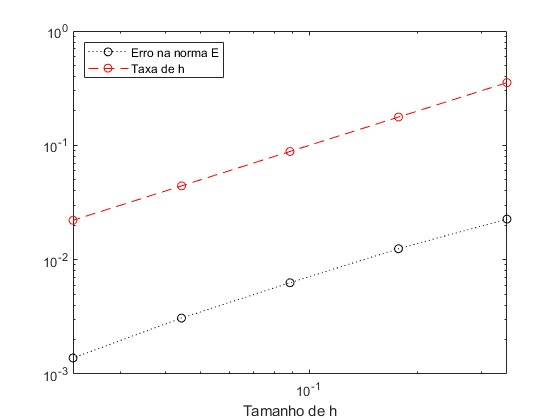
\includegraphics[scale=0.4]{2D_normE.jpg}
\caption{Gráfico \textbf{loglog} da norma $E$ na triangulação versus o tamanho de h. }
\end{figure}

\tab Desta forma, dado que, novamente, as retas apresentam o mesmo declive, é possível concluir que a norma $L^2$ se comporta como $Ch^2$ e que a norma de energia se comporta como $Ch$, o que vai de encontro aos resultados teóricos indicados nas secções 2.6 e 2.3. É também importante mencionar que a função auxiliar \verb +give_h(mesh)+ foi retirada das notas do Professor Antti
Hannukainen da Universidade de Aalto \textbf{[1]}.

\section{Comparação com o software \emph{FreeFEM}}

\tab Por motivos de curiosidade, compara-se as soluções obtidas do problema de Poisson em \textbf{2D} com as soluções obtidas no software grátis para análise do método dos elementos finitos chamado \emph{FreeFEM}. Para utilização desta ferramenta, usa-se o editor de texto disponível \href{https://freefem.org/tryit}{\textcolor{blue}{online}} e o compilador disponibilizado para \href{https://github.com/FreeFem/FreeFem-sources/releases}{\textcolor{blue}{download}}. O código usado neste projeto é apresentado tanto em formato .edp, para visualização através da aplicação \emph{FreeFEM}, e em formato .txt, para modificações futuras na IDE do \emph{website}.

\tab Começa-se por discretizar o domínio $\Omega$, de formato L, dentro do quadrado $ [0,1] \times [0,1] $, e a função fonte $f(x,y)=x^2$. Para tal, em línguagem \emph{FreeFEM}, é necessário definir as fronteiras usando o comando \verb +border+ e, subsquentemente, utilizar o comando \verb +buildmesh+ para construir a malha. A solução é calculada através do \emph{built-in solver} do software. Para se traçarem as fronteiras recorre-se ao uso de condições, isto é, definir intervalos para os valores $x$ e $y$ com uma dada orientação (é necessário que a orientação seja tal que é possível percorrer o perímetro). Efetivamente, é somente necessário escrever \verb +border+ seguido de um nome e um intervalo de valores para $t$. Subsequentemente, iguala-se ora $x$ ora $y$ a $t$ (consoante o valor que se pretende alterar) e o restante a uma constante. Neste caso, constrói-se uma fronteira em formato de L. É de realçar que o sentido é ditado da esquerda para a direita.  O seguinte código ilustra o processo.

\vspace{5mm}

\begin{lstlisting}[frame=single]
real error = 0.1;

func f = (x^2);
func g = 0.;

int NAdapt = 10;
 
// Malha
border ba(t=-1, 1){x=t; y=-1; label=1;}
border bb(t=-1, 1){x=1; y=t; label=1;} 
border bc(t=1, 0){x=t; y=1; label=1;} 
 
border bd(t=1, 0){x=0; y=t; label=1;}
border be(t=0, -1){x=t; y=0; label=1;}
border bf(t=0, -1){x=-1; y=t; label=1;}


plot(ba(4) + bb(4) + bc(4) + bd(4) + be(4) + bf(4));

mesh Th = buildmesh(ba(6) + bb(4) + bc(4) + bd(4) + be(4) + bf(6));

plot(Th);

fespace Vh(Th, P1);
Vh u, v;
 

// Problema
problem Poisson(u, v, solver=CG, eps=1.e-6)
    = int2d(Th)(
         dx(u)*dx(v)
       + dy(u)*dy(v)
    )
    - int2d(Th)(
         f*v
    )
    + on(1, u=0);
 
 

// Adaptmesh loop
for (int i = 0; i < 4; i++){
    Poisson;
    Th = adaptmesh(Th, u, err=error);
    error = error/2;
 } 

// Plot
plot(u);
\end{lstlisting}

\vspace{1mm}

\tab Usando os comandos de visualização do \emph{FreeFEM} é possível obter comparações com os gráficos obtidos por \emph{MATLAB}:

\vspace{5mm}

\begin{figure}[H]
\centering
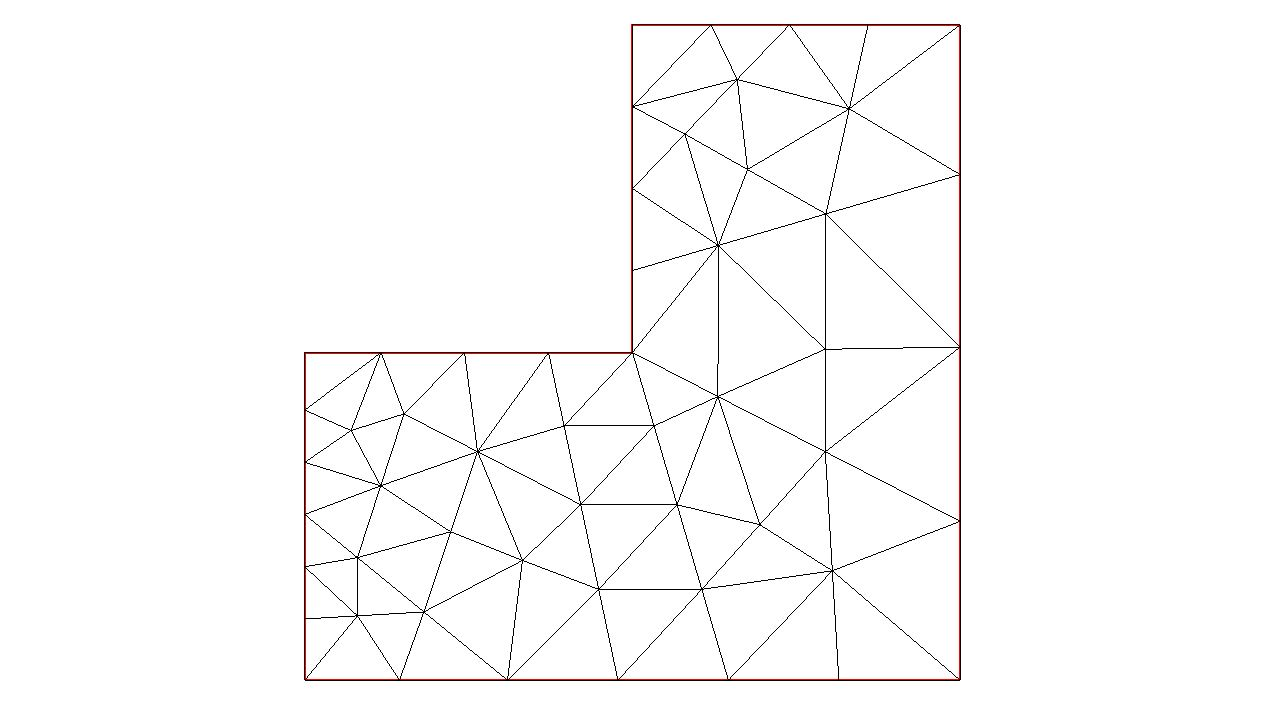
\includegraphics[scale=0.2]{malha_LFree.JPG}
\caption{O domínio $\Omega$ e a sua respetiva triangulação no \emph{FreeFem}.}
\end{figure}



\begin{figure} [H]
\centering
\begin{minipage}{0.4\textwidth}
  \centering
  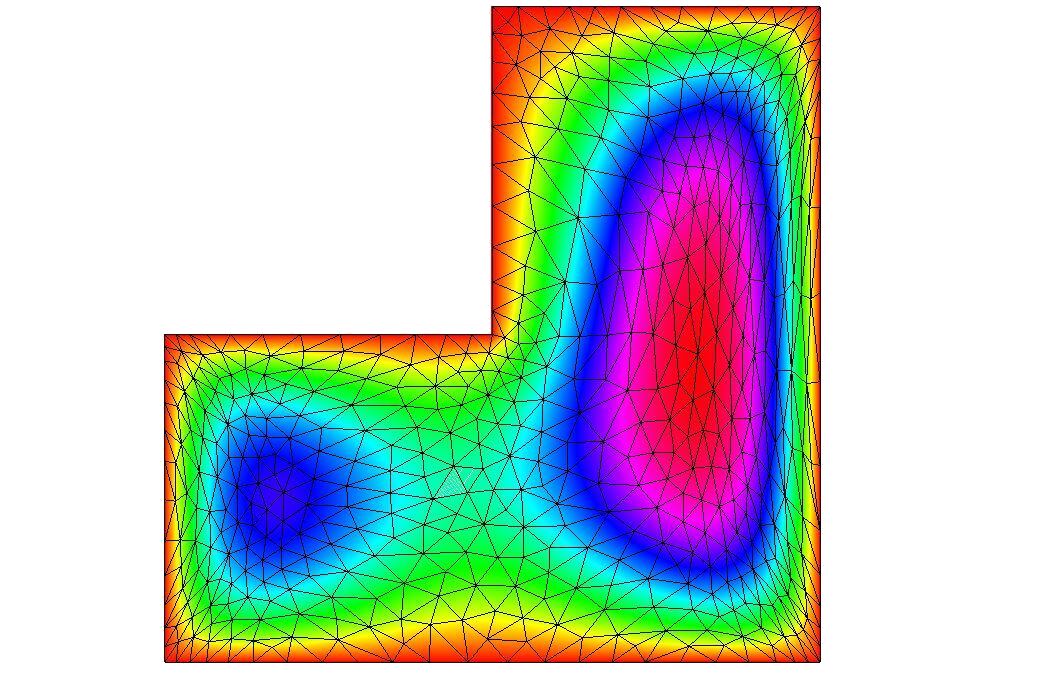
\includegraphics[height=4.0cm,width=1\linewidth]{bird_eye_view.png}
\end{minipage}%
\begin{minipage}{0.4\textwidth}
  \centering
  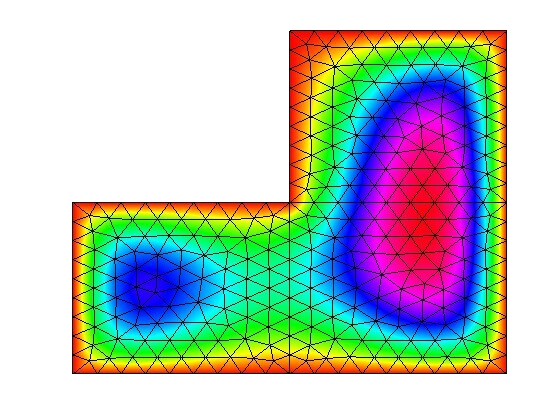
\includegraphics[height=4.7cm,width=0.85\linewidth]{bird_eye_view_mat.png}
\end{minipage}
\caption{Solução MEF  usando o software \emph{FreeFEM} (à esquerda) versus solução \emph{MATLAB} (à direita).}
\end{figure}

\begin{figure} [H]
\centering
\begin{minipage}{0.4\textwidth}
  \centering
  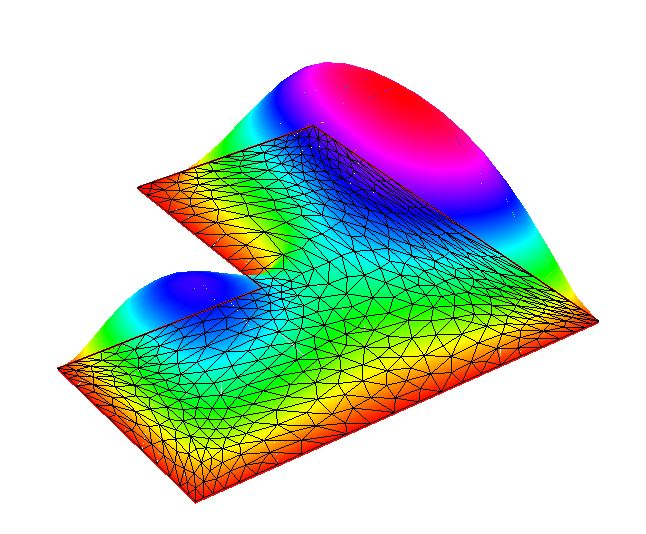
\includegraphics[height=5cm,width=0.7\linewidth]{3D_view.JPG}
\end{minipage}%
\begin{minipage}{0.4\textwidth}
  \centering
  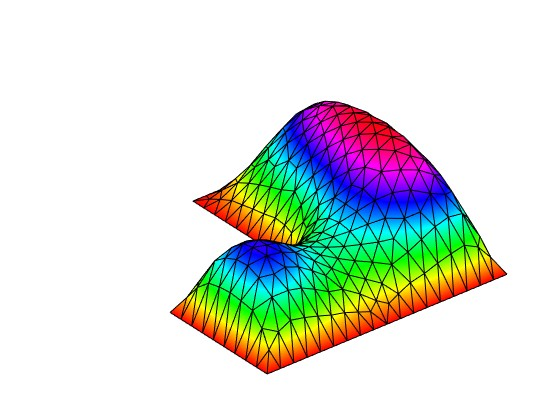
\includegraphics[height=6cm,width=0.9\linewidth]{3D_view_mat.jpg}
\end{minipage}
\caption{Visualização 3D MEF (à esquerda) usando o software \emph{FreeFEM} versus visualização \emph{MATLAB} (à direita).}
\end{figure}

\tab Como se pode observar nas Figuras 18 e 19, as soluções obtidas são bastante semelhantes. No entanto, devido ao facto de ser baseada na linguagem de programação \emph{C++}, o software \emph{FreeFEM} é mais rápido a compilar.

\tab Escolhendo ainda outro domínio $\Omega:=[0,1]\times[0,1]$, é possível obter comparações para a função fonte $f(x,y)=2y(1-y)+2x(1-x)$. Para tal basta alterar no \emph{script} anterior as fronteiras do domínio. Desta forma, temos simplesmente:

\vspace{1mm}
\begin{lstlisting}[frame=single]
border ba(t=0, 1){x=t; y=0; label=1;}
border bb(t=0, 1){x=1; y=t; label=1;} 
border bc(t=1, 0){x=t; y=1; label=1;} 
border bd(t=1, 0){x=0; y=t; label=1;}
\end{lstlisting}

\vspace{1mm}
\begin{figure} [H]
\centering
\begin{minipage}{0.4\textwidth}
  \centering
  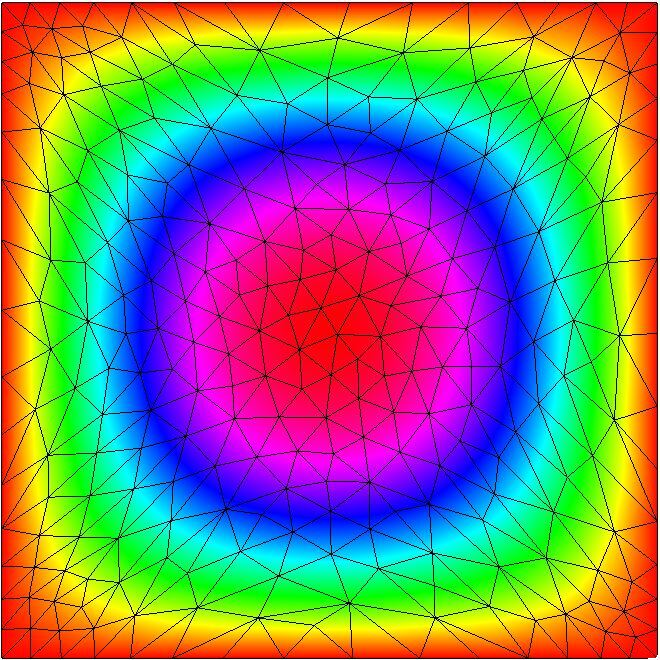
\includegraphics[height=3.7cm,width=0.7\linewidth]{bird_eye_view_quadrado.png}
\end{minipage}%
\begin{minipage}{0.4\textwidth}
  \centering
  \vspace{1.5mm}
  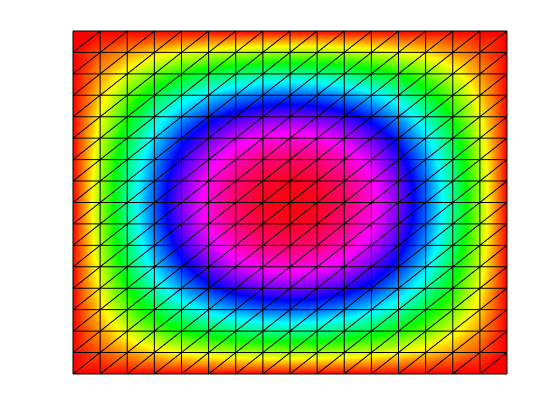
\includegraphics[height=4.7cm,width=0.9\linewidth]{bird_eye_view_quadrado_mat.png}
\end{minipage}
\caption{Solução MEF usando o software \emph{FreeFEM} (à esquerda) versus solução \emph{MATLAB} (à direita).}
\end{figure}

\vspace{1mm}
\begin{figure} [H]
\centering
\begin{minipage}{0.4\textwidth}
  \centering
  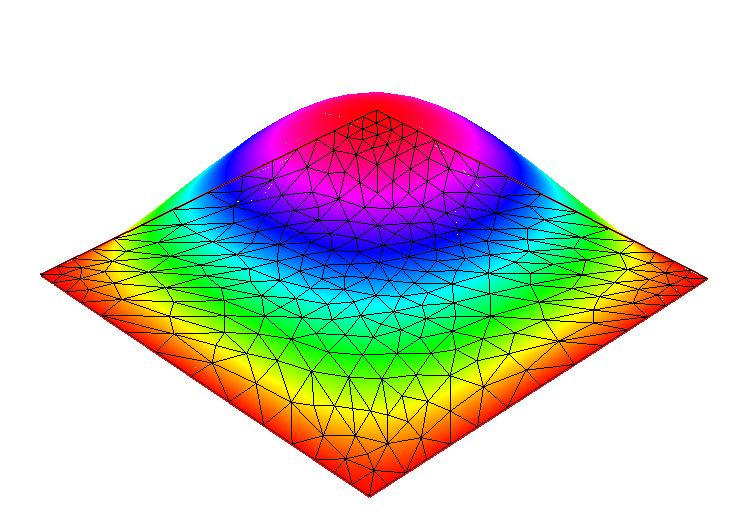
\includegraphics[height=4.7cm,width=0.7\linewidth]{3D_view_quadrado.JPG}
\end{minipage}%
\begin{minipage}{0.4\textwidth}
  \centering
  \vspace{1.5mm}
  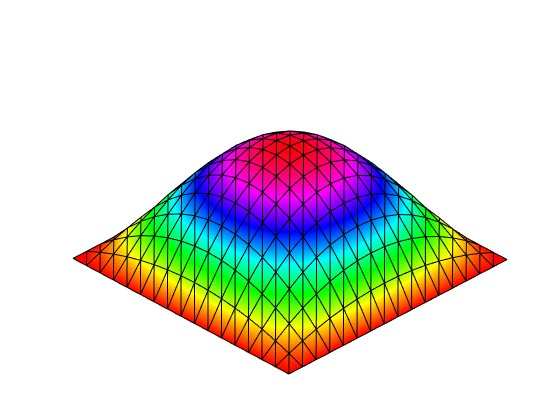
\includegraphics[height=5.7cm,width=0.9\linewidth]{3D_view_quadrado_mat.jpg}
\end{minipage}
\caption{Visualização 3D MEF usando o software \emph{FreeFEM} (à esquerda) versus visualização \emph{MATLAB} (à direita).}
\end{figure}

\vspace{1mm}

\tab Olhando para as Figuras 20 e 21, conclui-se  que as soluções são praticamente idênticas, as pequenas diferenças resultam de malhas algo diferentes. Outro benefício da utilização do \emph{FreeFEM} é a possibilidade de utilizar elementos de ordem superior a um. Para tal, basta alterar o parâmetro $P1$ na função \emph{fespace}.

\section{Conclusão}

\tab A aproximação da solução da equação de Poisson, tanto no caso \textbf{1D} como em \textbf{2D}, necessitou, primeiramente, da sua formulação em forma fraca, traduzindo-se o problema em forma variacional. Seguidamente, foi feita uma discretização do domínio $\Omega$ e escolha de bases seccionalmente polinomiais (lineares ou quadráticos), permitindo a tradução do problema num sistema de equações lineares. Finalmente, e após solução do sistema, foram observados os erros empíricos e a sua   respetiva convergência em função de h, tamanho da malha, confirmando-se as estipulações teóricas. Adicionalmente, somente para o caso $\textbf{1D}$, foi analisado o elemento de segunda ordem, construído através da introdução de uma função bolha, verificando o seu efeito na diminuição do erro entre a solução aproximada e a solução exata. Paralelamente, foi ainda possível estabelecer uma comparação entre o \emph{solver MATLAB}  desenvolvido ao longo do trabalho e as soluções obtidas através do uso de um \emph{software} próprio para a aplicação do método dos elementos finitos, o \emph{FreeFEM}.

\tab Em suma, este projeto serve como ilustração da aplicação do método dos elementos finitos a uma equação diferencial parcial, a equação de Poisson, analisando-se discretizações tanto no caso unidimensional como no caso bidimensional. Desta forma, o objetivo do projeto foi concluído, visto que foi possível a modelação da equação de Poisson e a construção de um ponto de partida para a resolução de outras E.D.P's, demonstrando-se a sua utilidade futura.



\section{Apêndice Matemático}
\tab Nesta secção são introduzidas noções teóricas extra que servem de base para a secção dos conceitos teóricos no início do relatório. Foi decidida criar esta secção não só para o interessado como para não interromper a fluidez do desenvolvimento teórico e, sobretudo, porque estes resultados não estão diretamente associados à implementação do método.
    
\subsection{Espaços de Sobolev}
\tab Antes de definir formalmente este tipo de espaços, é necessário introduzir a ideia de derivada fraca, isto é, procura-se extender a definição de derivada para funções que não são diferenciáveis num sentido clássico. Para tal, observa-se que o valor do integral não depende do comportamento da função integrada num conjunto finito de pontos, dado que um ponto tem medida nula. Relembrando a fórmula de integração por partes e definindo $L^1_{loc}(I)$ como sendo o espaço de funções que são Lebesgue integráveis em todo o subconjunto compacto de I; diz-se que $u \in L^1_{loc}(I) $ é fracamente diferenciável se existe $v \in L^1_{loc}(I) $ tal que $\int_I v \cdot \varphi \; dx = -\int_I  u \cdot \varphi' \; dx$ para todo o $\varphi \in C^\infty_0(I)  $. Assim é generalizado o conceito de derivada para funções que são somente Lebesgue integráveis, podendo não ser diferenciáveis, ou seja, a derivada fraca é definida em quase todo o $I$. Adicionalmente, uma função $u$ é $n$-vezes fracamente diferenciável se a sua $(n-1)$-ésima derivada fraca for fracamente diferenciável.

\tab Um espaço de \emph{Sobolev} é obtido definindo o espaço $H^m (I) \subset L^2(I)$ como sendo aquele cujos elementos são as funções $m$-vezes fracamente diferenciáveis munidas de produto interno dado por $(u,v)_{H^m(I)}=\sum^m_{k=0}(\frac{d^ku}{dx^k},\frac{d^kv}{dx^k})_{L^2(I)}$ e norma $\norm{u}=\sqrt{(u,v)_{H^m(I)}}$. É também importante definir a semi-norma de $H^m(I)$ dada por $|u|_{H^m(I)}:=\norm{\frac{d^\left(m\right)u}{dx^\left(m\right)}}_{L^2}$. Em \textbf{1D} as funções no espaço $H^1(I)$ são contínuas e portanto as fronteiras estão bem definidas. Desta forma, definimos o nosso primeiro espaço de Sobolev $H_0^1:=\{u \in H^1(I) \; | \; u(a)=u(b)=0\}$. É de notar que $|u|_{H^1(I)}$ define uma norma em $H^1_0(I)$ e que o espaço $H^1(I)$ é composto de funções quadrado integráveis cuja primeira derivada é também de quadrado integrável.

\subsection{Problema variacional e existência de solução única}
\label{sec:7.3}
\tab Considere o seguinte problema variacional: encontrar $u \in V$  que satisfaz $a(u,v) = L(v) $ $\forall v \in V$, em que $V$ é um espaço de Hilbert com norma $\norm{\cdot}_V$, $a$ é uma aplicação $V \cross V \to \R$  bilinear e $L$ é uma aplicação $V \to \R$ linear. Supõe-se ainda que a forma bilinear a e a forma linear L satisfazem as seguintes propriedades:
\vspace{3mm}
\begin{itemize}
    \item Continuidade de $a$: $a(u,v)\leq C\norm{u}_V\norm{v}_V$
    \item Elipticidade de $a$: $a(u,u)\geq \alpha\norm{u}^2_V$
    \item Continuidade de $L$: $|L(V)|\leq C_L\norm{v}_V$
\end{itemize}
\vspace{3mm}
em que $C, \alpha$ e $C_L$ são constantes positivas independentes de $u$ e $v$. 

\tab Agora define-se o teorema principal desta secção e que é fundamental para a prova da existência de solução única para o problema de Poisson.

\vspace{1mm}

\textbf{Teorema} (Teorema de Lax-Milgram): Seja $a$ uma aplicação bilinear dotada de continuidade e elipticidade e $L$ uma aplicação limitada. Então existe um e um só $u \in V$ tal que $a(u,v) = L(v) $ $\forall v \in V$, isto é, é solução do problema variacional.

\vspace{1mm}

\textbf{Corolário}: O problema de Poisson tem solução única.

\vspace{1mm}

\textbf{Dem:}

\vspace{1mm}
A demonstração faz-se por prova sucessiva das propriedades. Apresenta-se a prova apenas no caso \textbf{1D}.

\textbf{Continuidade de $a$}: Para mostrar a continuidade do problema de Poisson em \textbf{1D} tem que se provar que:

\begin{equation*}
    a(u,v) \leq \norm{u}_{H^1}\norm{v}_{H^1}
\end{equation*}


Efetivamente, pela desigualdade de Cauchy-Schwarz vem:
\begin{equation*}
     \abs{a(u,v)}=\abs{\int^1_0\frac{du}{dx}\frac{dv}{dx}}=\abs{(u',v')_{L^2(I)}} \leq \norm{u'}_{L^2(I)}\norm{v'}_{L^2(I)}
\end{equation*}

Adicionalmente, repare-se que $\norm{w}_{H^1(0,1)}:=\left(\norm{w}^2_{L^2(I)}+\norm{w'}^2_{L^2(I)}\right)^{\sfrac{1}{2}}$. Como $\norm{w}_{L^2(I)} \geq 0$ então é claro que $\norm{w'}_{L^2(I)} \leq \norm{w}_{H^1(0,1)}$. Portanto, temos o resultado pretendido.

\vspace{1mm}

\textbf{Elipticidade de $a$:}

A elipticidade requer um resultado adicional chamado desigualdade de Poincaré-Friedrichs. Efetivamente dado $I=(a,b)$ e definindo $s=b-a$ então existe uma constante $C_P>0$ tal que:

\begin{equation*}
    \norm{v}_{L^2(I)} \leq C_P \norm{v'} _{L^2(I)}  \; \; \forall v \in H^1_{0}(I)
\end{equation*}

Por definição:

\begin{equation*}
    a(u,u)=\int^1_0 (u')^2 \; dx = \norm{u'}_{L^2(I)}
\end{equation*}

E também é verdade que $\norm{u'}_{L^2(I)}=\frac{1}{2}\norm{u'}_{L^2(I)}+\frac{1}{2}\norm{u'}_{L^2(I)}$. Usando a desigualdade apresentada acima então $\frac{1}{2}\norm{u'} _{L^2(I)} \geq \frac{1}{2C_P}\norm{u}_{L^2(I)} $. Logo:

\begin{equation*}
 \norm{u'}^2_{L^2(I)} \geq \frac{1}{2}\norm{u'}^2_{L^2(I)} + \frac{1}{2C_P}\norm{u}^2_{L^2(I)} \geq \min\left\{{\frac{1}{2},\frac{1}{2C}}\right\}\left(\norm{u'}^2_{L^2(I)} + \norm{u}^2_{L^2(I)}\right)
\end{equation*}

E então a condição de elipticidade é cumprida para $\alpha=\min\left\{{\frac{1}{2},\frac{1}{2C}}\right\}$.

\vspace{1mm}

\textbf{Continuidade de $L$:}

Usando novamente a desigualdade de Cauchy-Schwarz:
\begin{equation*}
    \abs{L(v)}=\abs{\int_I fv \; dx}=\abs{(f,v)_{L^2(I)}} \leq \norm{f}_{L^2(I)} \norm{v}_{L^2(I)} \; \;\forall v \in H^1_0(I)
\end{equation*}

Como $\norm{v}_{L^2(I)} \leq \norm{v}_{H^1}$ a condição é satisfeita.

\subsection{Resultados sobre interpolação}
\label{sec:7.5}
\tab Considerando uma função contínua $w$ e uma função $\pi w$ que interpola essa mesma função nos nós $\{x_1,...,x_n\}$, contínua e linear em cada intervalo de partição $I_j=[x_j,x_{j+1}]$ tal que $\pi w(x)=\sum^N_{j=1}w(x_j)\hat{\varphi}_j(x)$ então é possível estabelecer as seguintes desigualdades;
\begin{equation*}
    \norm{w-\pi w}_{L^2(I)} \leq h^2\norm{w''}_{L^2(I)},
\end{equation*}
\begin{equation*}
    \norm{(w-\pi w)'}_{L^2(I)} \leq h\norm{w''}_{L^2(I)}.
\end{equation*}

\vspace{3mm}

\section{Bibliografia}
\textbf{[1]}  Hannukainen, A., Finite Element Method, Lecture Notes,
Universidade Aalto, 2021.

\vspace{1mm}
\textbf{[2]}  Larson, M.G, e F. Bengzon, The Finite Element Method: Theory,
Implementation, and Applications, Springer, 2013.

\vspace{1mm}

\vspace{1mm}
\textbf{[3]}  Videman, J., Matemática Computacional, Aula XX, Departamento de Matemática, IST, 2021

\vspace{1mm}

\textbf{[4]} Link para IDE:  \href{https://freefem.org/tryit}{\textcolor{blue}{https://freefem.org/tryit}}

\vspace{1mm}
\textbf{[5]} Link para compilador:
\href{https://github.com/FreeFem/FreeFem-sources/releases}{\textcolor{blue}{https://github.com/FreeFem/FreeFem-sources/releases}}
\end{document}